\chapter{Methodology}
\section{Conceptual Framework}\label{sec:research-design}
The study has two mutually connected, but experimentally distinct, phases. Phase I develops and evaluates a controlled text-classification artifact without requiring sensitive resident complaints. Phase II describes how that artifact would support a human-governed barangay reporting system. The separation is essential: achieving a test-set score completes a model experiment, whereas operating a public-facing reporting system requires application, governance and safety verification. Figure~\ref{fig:overall} presents these phases with an explicit release gate and a feedback loop that returns reviewed corrections to \emph{offline} retraining instead of changing a live classifier automatically.
\begin{figure}[H]\centering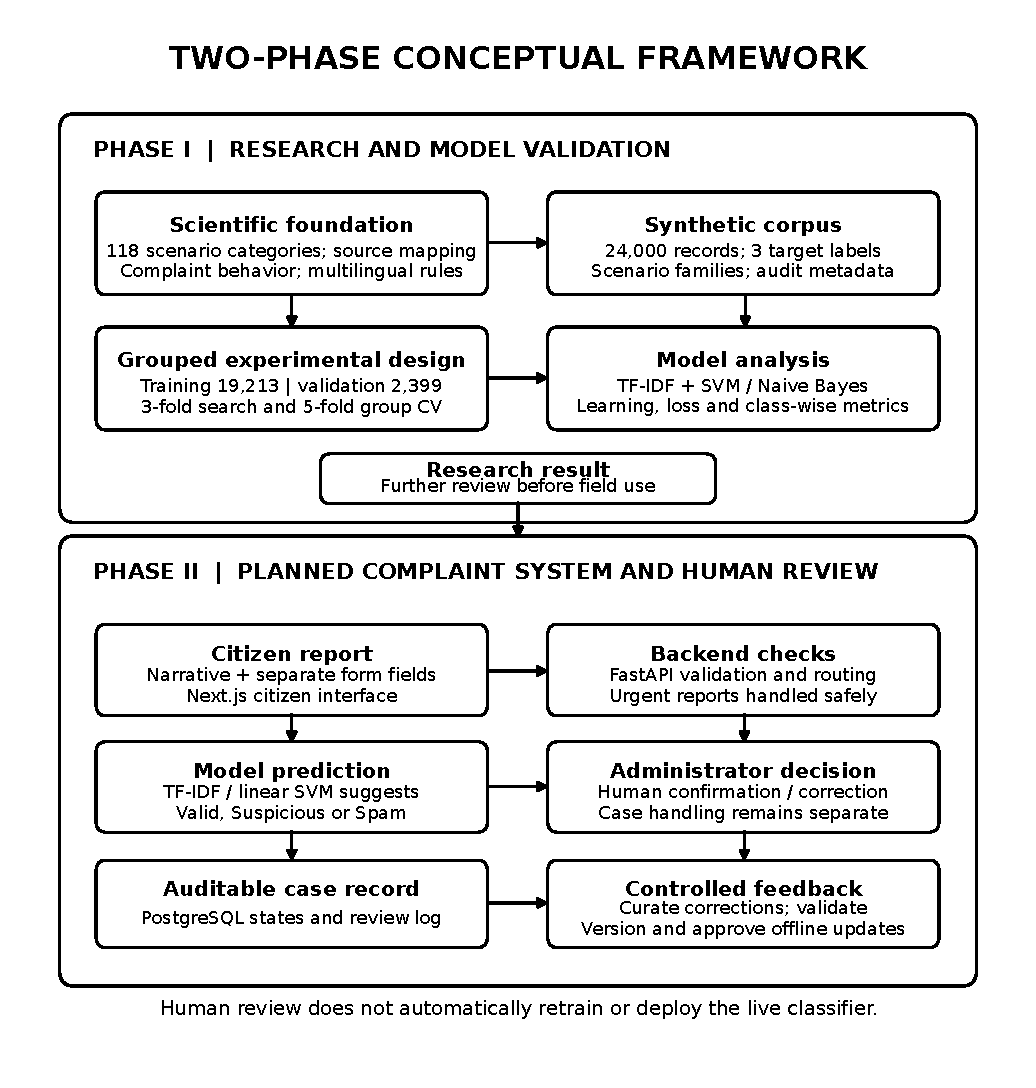
\includegraphics[width=0.96\textwidth,height=0.85\textheight,keepaspectratio]{figures/conceptual_framework.pdf}\caption{Expanded two-phase conceptual framework separating research preparation, model selection, provisional inference, human review and controlled feedback. Arrows distinguish the measured research workflow from the proposed operational workflow; administrator feedback is reviewed offline rather than automatically deployed.}\label{fig:overall}\end{figure}
\subsection{Phase I: Evidence-Based Corpus Development}
The offline phase begins with a source register: national legislation provides examples of community responsibility and safeguards, local reporting guidance describes information useful for incident review, linguistic studies inform complaint speech acts and code-switching, and synthetic-data research informs variation and evaluation controls. These sources \emph{inform} the scenario design. They do not certify each generated sentence as authentic or prove that the proportions are representative. A 118-item researcher-defined taxonomy supplies 60 Valid issue topics, 28 Suspicious clarification reasons and 30 Spam types. Each item receives an explicit scope definition, an intended three-class label, and references to the corresponding evidence type.

The generation stage distinguishes \emph{scenario meaning} from \emph{surface form}. A hypothetical clogged-drain concern can be written as an informal question or a detailed narrative without changing its class. A confusing report may instead refer only to ``the thing I reported before'' with no recoverable subject. A promotional solicitation lacks a community grievance altogether. Generator logic chooses a controlled language group, communication form, narrative length and contextual cues, then constructs the sentence. Every output carries source traceability, seed, topic/review/spam identifier and a scenario family. These metadata fields are excluded from the text-only classifier. Figure~\ref{fig:dataset} details this process.
\begin{figure}[H]\centering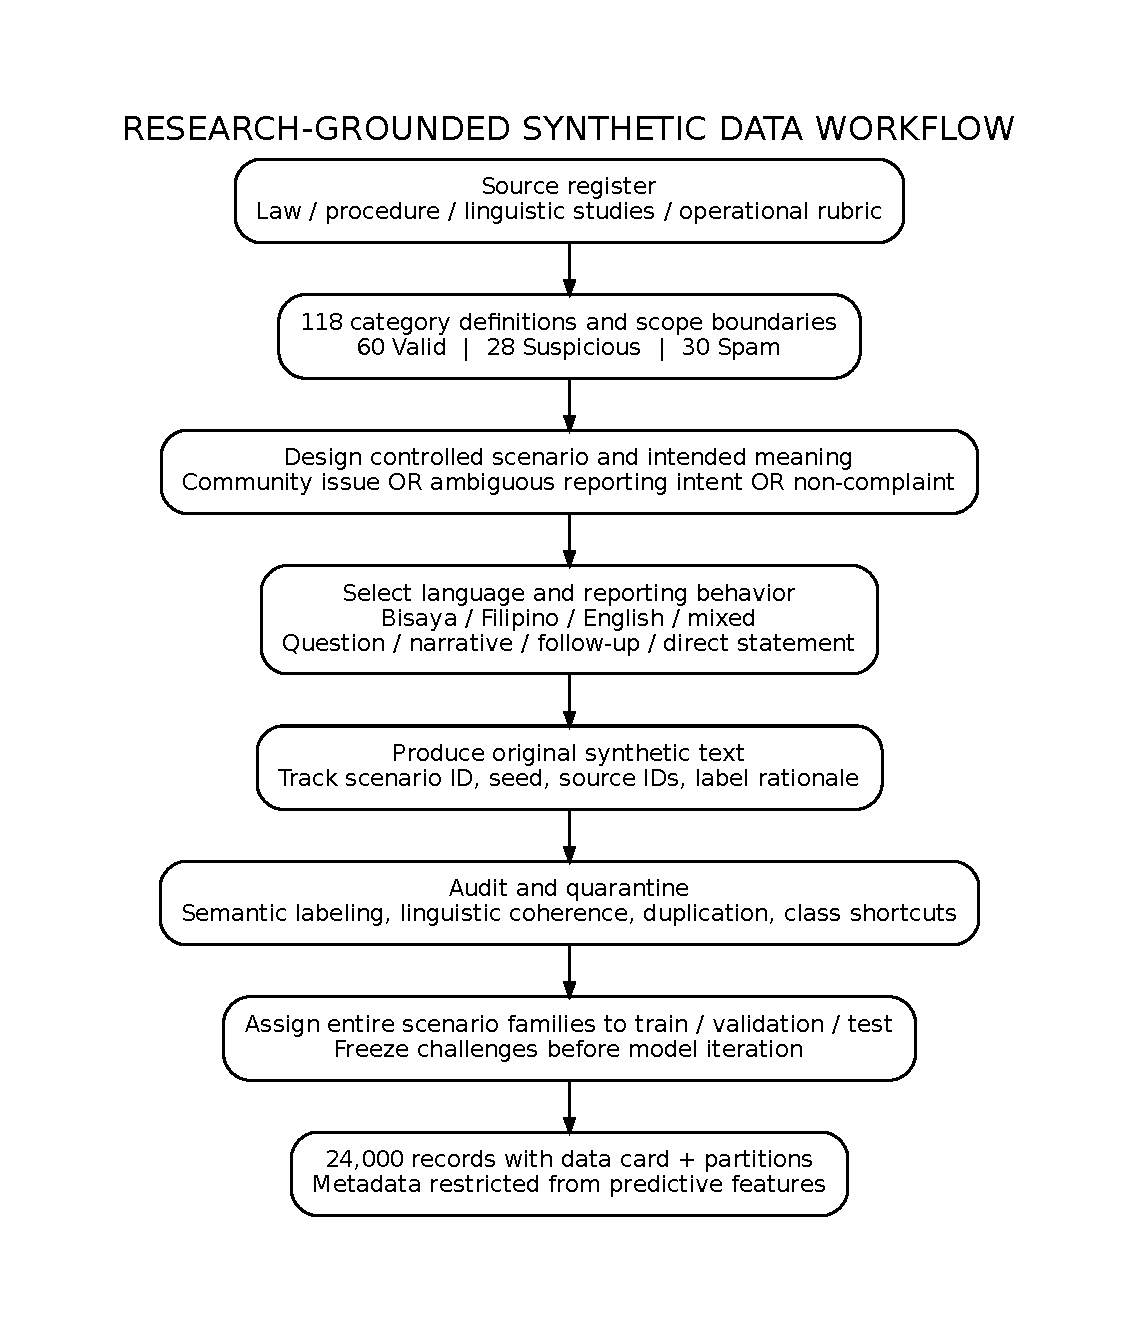
\includegraphics[width=0.94\textwidth,height=0.82\textheight,keepaspectratio]{figures/dataset_pipeline.pdf}\caption{Scenario-first data construction and audit pipeline. The label is based on intended communicative meaning, not on incidental length, grammar, sentiment, or language.}\label{fig:dataset}\end{figure}
\subsection{Phase II: Proposed Public Reporting Service}
The proposed operational system separates resident input, inference, administrative review, case management, and controlled model maintenance. A resident-facing form collects a required Subject and Complaint Details narrative; incident date/time and Purok/Sitio or an identifying landmark are supporting contextual fields when known. Geographic maps, GPS capture and photographic uploads are outside the selected core thesis scope. The application concept uses an authenticated resident interface and an authorized staff interface; the suggested software stack is Next.js/TypeScript, FastAPI and PostgreSQL, but implementation claims require working source code and testing. No completed user-interface or government-office deployment evaluation is included in the supplied experimental evidence.

The class-prediction output is separate from the administrative disposition. Predicted Valid goes to the accepted-case workflow under the selected routing rule; predicted Suspicious or Spam goes to administrator review. Acceptance, clarification, and rejection are decisions about the submission, not automatic replacements for the text label. Proposed controls include resident status tracking, staff action logs, deadline monitoring, referrals, verification before resolution, and a reconsideration mechanism. Detailed proposed figures and the experimental--operational boundary are presented later in this chapter.

\section{Descriptive Analysis of the Dataset}
\label{sec:data-description}
This section updates the study's earlier data-description protocol to reflect the corpus actually used for the reported experiments. The study originally considered de-identified administrative archives, subject to access approvals, and supplemental simulated examples. Those were possible acquisition pathways, not completed observations. The experimental data currently consist entirely of \emph{researcher-constructed synthetic complaint narratives}; no authentic barangay records are presented as training data. The objective of using controlled synthetic text is to build an auditable and systematically varied classification benchmark, not to estimate how frequently a complaint type occurs in Davao City. Following Chicco et al.~\cite{chicco2022} and Bender and Friedman~\cite{benderfriedman}, the data's provenance, sampling choices, missing coverage and preprocessing choices are reported alongside model scores.

\subsection{Data Sources, Construction and Composition}
Source acquisition in this study refers to researching the \emph{foundations of scenario design}: Philippine barangay governance and topic-specific laws, administrative reporting guidance, studies of Filipino complaint speech acts and code-switching, and published approaches to spam and synthetic-text validation. Each of 60 Valid topics, 28 Suspicious review reasons and 30 Spam forms is tracked in the accompanying source-to-category matrix. These references provide topic or linguistic justification; they neither certify individual generated incidents as real nor imply the 118 categories are official government labels. Generation was carried out from researcher-designed incident descriptions and style frames; the existing fixed corpus is not being regenerated in this revision.

The corpus contains \textbf{24,000} records and \textbf{21 recorded fields}. Of those, the predictive input is \texttt{complaint\_text} and the target is \texttt{classification}. Supporting columns record category, language assignment, scenario or template family, provenance, assigned partition, and review-status flags. The raw unmodified CSV remains preserved within the research repository. All 24,000 source-type entries are marked \texttt{synthetic\_researcher\_constructed\_unreviewed}. This label distinguishes the corpus from real archived reports and from independently annotated gold-standard data.

\begin{table}[H]\centering\caption{Observed corpus composition and provenance}\label{tab:m1composition}\small
\begin{tabularx}{\textwidth}{p{0.42\textwidth}rX}\toprule
\textbf{Dimension} & \textbf{Records} & \textbf{Interpretation}\\\midrule
Entire research corpus & 24,000 & 100\% researcher-generated synthetic text\\
Valid & 8,000 & 33.33\% of corpus\\
Suspicious & 8,000 & 33.33\% of corpus\\
Spam & 8,000 & 33.33\% of corpus\\
Bisaya/Cebuano (assigned) & 6,000 & 25\% of corpus\\
Filipino (assigned) & 6,000 & 25\% of corpus\\
English (assigned) & 6,000 & 25\% of corpus\\
Mixed/code-switched (assigned) & 6,000 & 25\% of corpus\\
Verified human annotations & 0 & No independent label review recorded\\
Authentic archived complaints & 0 & Not a sampled administrative archive\\\bottomrule
\end{tabularx}\end{table}

\subsection{Exploratory Data Analysis and Text Characteristics}
Exploratory Data Analysis (EDA) was computed on the existing unprocessed \texttt{complaint\_text} values using whitespace-delimited word counts, class totals, assigned language totals and duplicate checks. Token length in this table is a reproducible whitespace-word count, not a universal measure of syllables or morphologically segmented Cebuano vocabulary. The corpus has no missing complaint narrative and no exact duplicate strings, but neither condition rules out meaning-equivalent paraphrases, repeated phrasal openings or near-duplicate source patterns.
\begin{table}[H]\centering\caption{Measured narrative lengths by supervisory label}\label{tab:m1lengths}\small\begin{tabular}{lrrrrr}\toprule
\textbf{Label} & \textbf{$n$} & \textbf{Mean} & \textbf{Median} & \textbf{Minimum} & \textbf{Maximum}\\\midrule
Valid & 8,000 & 20.76 & 20 & 5 & 48\\
Suspicious & 8,000 & 29.78 & 28 & 8 & 66\\
Spam & 8,000 & 14.90 & 15 & 1 & 35\\\bottomrule
\end{tabular}\end{table}
The overall corpus has a mean length of 21.81 words, median of 21 words, and observed range of 1--66 words. Figure~\ref{fig:m1lengths} displays the unequal within-class distributions. Suspicious entries average substantially longer than Spam, showing that an initially balanced class design can still encode unintended class cues in narrative length. This motivates the length-only and character-ngram diagnostics reported in Chapter~4; equal class totals alone cannot prevent superficial shortcuts.
\begin{figure}[H]\centering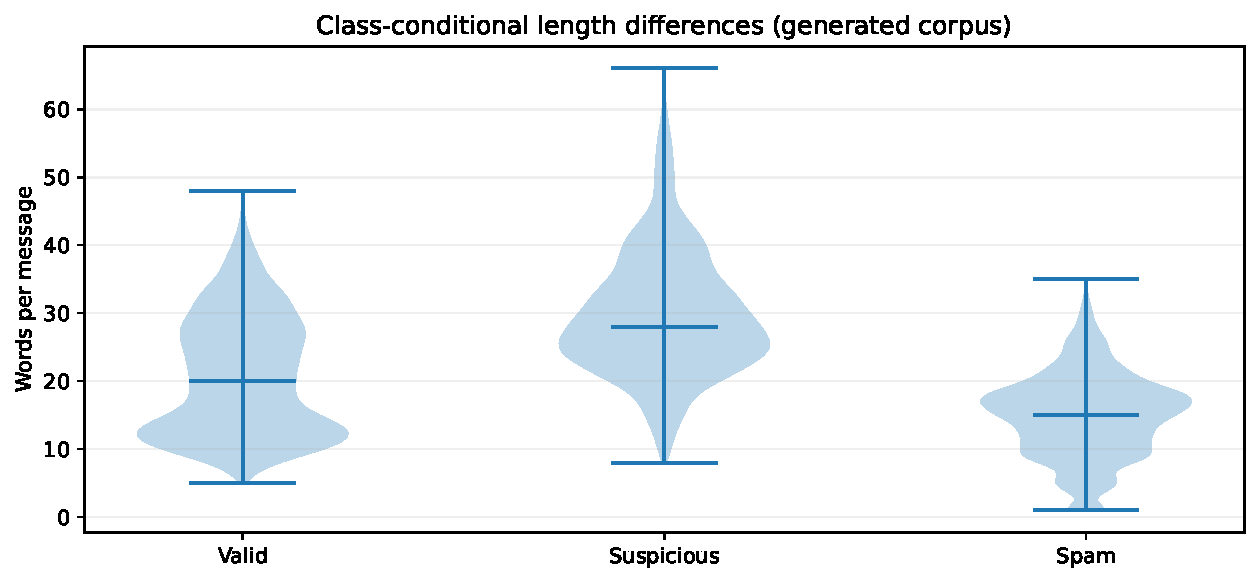
\includegraphics[width=.86\textwidth]{figures/m1_length_violin.pdf}\caption{Class-wise generated narrative length distributions, showing that equal class counts do not imply equal wording characteristics.}\label{fig:m1lengths}\end{figure}
The data were organized into 19,213 training, 2,399 validation and 2,388 test entries (80.05\%, 10.00\% and 9.95\%, respectively after rounding). Small deviations from a nominal 80/10/10 allocation arise from assigning shared scenario-family IDs to the same partition. This actual partition replaces the earlier \emph{proposed} stratified 80/20 train--test arrangement; neither design should be simultaneously presented as implemented. Neither the assigned language proportions nor the target-class proportions are estimates of demographic or reporting-channel prevalence.

\subsection{Inherent Biases, Sampling Gaps and Residual Risks}
Synthetic construction eliminates the need to treat past administrative acceptance or rejection decisions as ground truth, but introduces different biases. \emph{Selection bias} arises because researchers choose the 118 scenarios, seed incidents and forms of ambiguity, which may omit types of future complaints. \emph{Generator-pattern bias} arises from repeated frames, vocabulary and length conventions. \emph{Language coverage bias} arises when Bisaya and mixed-language expressions are assigned evenly without verifying natural idiom or dialect variation. \emph{Annotation bias} arises because labels are applied by rule and no independent annotator agreement has yet been measured. \emph{Operational distribution shift} arises because real inputs could have different class base rates, spelling mistakes, topics, contextual references or user behaviors. \emph{Temporal drift} could affect slang, complaint topics and spam strategies after generation.

Unlike studies based on real administrative archives, this particular corpus cannot directly measure historical discrimination or exclusion \emph{within actual office records}, because no such records were sampled. Nevertheless, if the system later incorporates staff corrections, differences in administrator practice, submission channels, access to the internet and language preference could be reproduced through feedback. These risks must be audited separately rather than claimed as eliminated. Documentation of intended linguistic coverage and limitations follows the data-statement rationale in \cite{benderfriedman}.

\begin{table}[H]\centering\caption{Bias risks, recorded controls and remaining gaps}\label{tab:m1bias}\footnotesize
\begin{tabularx}{\textwidth}{p{.21\textwidth}p{.39\textwidth}X}\toprule
\textbf{Risk} & \textbf{Control already reflected in corpus / experiments} & \textbf{Residual validation need}\\\midrule
Class imbalance & Deliberate 8,000/8,000/8,000 allocation & Test differing real-world base rates\\
Language imbalance & Four equal generator-assigned groups & Fluent-speaker and sub-language review\\
Labeling subjectivity & Written three-class rubric, 118 source-linked reasons/topics & Blind dual annotation, Cohen's kappa\\
Exact duplication & No exact repeated narrative among 24,000 records & Check near duplicates, shared seed syntax\\
Partition leakage & Scenario-family group separation; fold-only TF-IDF fitting & Test unrelated root-seed and writing-family holdouts\\
Generator shortcuts & Length and feature-ablation diagnostics & More adversarial minimal-pair tests\\
Administrative bias & No past office disposition field used as model input & Audit reviewer corrections before retraining\\\bottomrule
\end{tabularx}\end{table}

\subsection{Cleaning, Preprocessing and NLP Representation}
The recorded pipeline uses the narrative as the \emph{sole predictive feature}. Basic import and integrity checks ensure required text is present and encoding can be read. Conservative normalization handles whitespace and case through the TF-IDF analyzer. Word tokenization and configurable unigram/bigram extraction construct sparse numeric vectors. The \texttt{TfidfVectorizer} is fitted \emph{inside each training fold} and then applied with \texttt{transform} to held-out data; fitting it before splitting would leak corpus vocabulary and term frequencies. Dataset category IDs, language assignments, complaint status and reported resolution are not used as predictive features. The distinct proposed preprocessing workflow is described in the operational-workflow section; the completed experiments use word TF--IDF rather than the combined word--character proposal.

The earlier methodology proposed stopword filtering, stemming and lemmatization as possible steps. None is asserted to have improved results or to have been deployed in the current final TF-IDF--SVM model: deleting Cebuano negation, particles or borrowed terms could remove meaning. Likewise, named-entity masking is a privacy measure for future user-submitted text, but the present corpus consists of fictional scenarios and does not constitute a verified de-identification evaluation. The project preserves raw text for auditability and fitted preprocessing objects for consistent later inference.
\subsection{Class Balancing, Curation and Overfitting Controls}
Because the recorded study set is \emph{already balanced by construction}, no minority-class oversampling or synthetic minority oversampling technique (SMOTE) was needed to create parity across Valid, Suspicious and Spam. The data-generation process itself is the curation/balancing intervention. SMOTE was \emph{not applied}: interpolation between high-dimensional sparse TF-IDF vectors might not correspond to interpretable complaint messages. Likewise, class-weighted SVM training and random oversampling were discussed as possible controls for future imbalanced feedback datasets, but should not be described as completed current experiments unless supported by run configurations. When comparing such methods in future, balancing must be restricted to the training data \emph{inside} validation folds, never applied to held-out validation or test samples.

Regularization is the model-appropriate overfitting control: the SVM penalty parameter $C$ was explicitly tuned over $\{0.1,1,10\}$. The TF-IDF n-gram range and minimum document frequency were also tuned as feature-complexity controls, with an upper document-frequency restriction and sublinear term-frequency weighting held fixed. Model selection used three-fold scenario-grouped cross-validation, supplemented with five-fold group-disjoint fixed-model diagnostics on the training partition; fixed validation performance and loss/learning curves are reported in Chapter~4. A linear SVM has no dropout layers, and the selected \texttt{LinearSVC} does not provide a neural-network-style early-stopping history. A separate SGD-based linear hinge-loss estimator supplied the reported epoch-level \emph{auxiliary} loss curves. Regularization and grouped validation reduce some forms of fit-related risk but cannot certify transfer to unseen generator root patterns.
\subsection{Human Annotation and Controlled Feedback}
The earlier research protocol proposed that Gonzaga and Badong independently annotate a calibration subset, reconcile disagreements and calculate Cohen's kappa \cite{artstein}. This remains an \emph{uncompleted validation procedure}; the corpus marks all records \texttt{human\_label\_reviewed=No}. The implemented annotation method is generator-rule labeling, not independently measured consensus. A future review sample should be stratified by all three classes, language groups, category families, length bands and deliberately ambiguous boundary cases. Reviewers should receive complaint text alone, without metadata revealing the intended label, and adjudication outcomes should be preserved.

The intended Human-in-the-Loop process similarly requires an administrator to confirm or correct a provisional prediction, with decisions stored for later audit. Such feedback does not imply that a deployed SVM continuously changes its weights in real time. Any proposed feedback dataset must be curated, its demographic/language distribution analyzed, and model updates separately trained, validated and versioned before approval. Neither improved live accuracy nor reduced administrative effort is claimed here without an evaluated deployment study. Residual bias and model-generalization gaps are discussed under Future Work in Chapter~5.


\section{Research Design and Research Questions}
The study uses applied, quantitative experimental design for its completed machine-learning work and system-design methodology for the proposed application. The primary output is an auditable three-class text classifier. The dependent variables are classification accuracy, precision, recall, Macro-F1 and subgroup errors; independent experimental choices include input language assignment, category family, textual length, message construction pattern, TF-IDF feature ranges and SVM regularization. No causal effect of human corrections is claimed until a frozen pre-update/post-update evaluation is performed.

\section{Corpus Construction and Provenance}
\subsection{Fixed Research Taxonomy and Label Boundaries}
The 118 categories are a scenario inventory and audit framework, not 118 machine-learning output classes. A Valid record conveys an understandable community-related concern or safety report, even if the barangay must refer it to another agency. Suspicious indicates essential context is missing, self-contradictory, or unrecoverably ambiguous \emph{from the input text}; it is not an accusation of dishonesty. Spam communicates no interpretable barangay-reporting purpose. Missing photographs, the absence of a name, nonstandard grammar, or anger alone do not warrant a Suspicious label. Reports \emph{about} scam incidents differ from scam solicitations \cite{ra7160,ra9262,ibanez}.
\begin{table}[H]\centering\caption{Three-class operational decision rubric}\small\begin{tabularx}{\textwidth}{p{0.21\textwidth}X}\toprule
\textbf{Class} & \textbf{Positive criterion and crucial exception}\\\midrule
Valid & Interpretable event, request or community concern. Short, emotional, anonymous and code-switched complaints may all be Valid.\\
Suspicious & Report-like wording but no recoverable issue, unresolved contradiction, or essential missing reference. It is a \emph{clarification state}, not a finding of falsity.\\
Spam & Promotional, impersonation or irrelevant submissions lacking citizen reporting intent; also nonsensical or classifier-directed text. A citizen reporting spam or scam activity can be Valid.\\\bottomrule
\end{tabularx}\end{table}

\subsection{Source-to-Category Traceability}
The evidence matrix bundled with the Overleaf project maps all 118 category IDs to laws, municipal complaint procedures, literature or researcher-defined rules. The mapping is deliberately qualified: statutes justify topics and jurisdictional context; linguistic papers justify forms of expression; and operational definitions justify unreported or undecidable content. An entry is not considered evidence that a specific synthetically generated narrative occurred in reality. Specialized domains involving violence, children, fraud, utilities and public danger must use appropriate referral practices. An appendix lists the category register used in generation.

\subsection{Generation Controls and Dataset Composition}
The released study corpus was produced with fixed random seed \texttt{20261026}. It contains exactly 24,000 unique text records: 8,000 per classification, and within each class 2,000 per generator-assigned language group (Bisaya, Filipino, English, Mixed). The generator uses researcher-authored source-aware scenario descriptions, reason-specific ambiguous seed messages and non-complaint examples, combined with structured variations in question forms, greetings, follow-up expressions, requested actions, partial location/time cues, emotional language and length bands. Every row is identified as synthetic and unreviewed; its assigned language is not independently verified. The equal distributions are experimentally controlled and cannot estimate true complaint prevalence.
\begin{table}[H]\centering\caption{Corpus structure and recorded partitions}\begin{tabularx}{\textwidth}{p{.43\textwidth}rX}\toprule
\textbf{Dimension}&\textbf{Count}&\textbf{Role}\\\midrule
Valid / Suspicious / Spam&8,000 each&Target labels\\
Bisaya / Filipino / English / Mixed&6,000 each&Generator allocation\\
Valid topics / Suspicious reasons / Spam types&60 / 28 / 30&Scenario metadata\\
Training&19,213&Fit features and select candidates\\
Validation&2,399&Model selection diagnostics\\
Synthetic test&2,388&Final within-generator estimate\\\bottomrule\end{tabularx}\end{table}

\subsection{Data Dictionary and Feature-Exclusion Boundary}
The predictive feature is \texttt{complaint\_text}; the supervised target is \texttt{classification}. Fields such as \path{category_id}, \path{source_reference_ids}, \path{scenario_family_id}, \path{template_family_id}, \path{language_group}, \texttt{split}, and \texttt{label\_rule} exist only for quality review and experimental controls. Feeding them to the SVM would directly expose the desired label or generation family and invalidate the intended text-only evaluation.

\section{Data Quality Assurance and Threats to Validity}
The generator removed exact-duplicate candidate outputs and verified nonempty narratives, target-class counts and category coverage. These technical checks do not establish natural idiom, correct meaning, grammatical coherence or independent annotation agreement. Accordingly the dataset retains flags marking \texttt{language\_verified=No} and \texttt{human\_label\_reviewed=No}. The remaining required manual assessment is an adjudicated stratified sample across 118 categories, three classes, four assigned languages, length bands and borderline pairs. At least two independent reviewers should code labels while blinded to generation metadata, adjudicate disagreements, and report agreement alongside confusion rates; a fluent Cebuano/Filipino review is essential before deployment claims. These are planned review tasks, not completed results.

\section{Experimental Setup and Models}
\subsection{Text Representation and Linear Models}
TF-IDF transforms the complaint narratives into a sparse feature space. Multinomial Naive Bayes serves as the baseline estimator using word unigrams/bigrams; the primary model is \texttt{LinearSVC} with regularization parameter $C$. Both operate solely on complaint narrative text, but their recorded TF--IDF settings are different: the Naive Bayes baseline uses word unigrams/bigrams whereas the chosen SVM uses word unigrams. Thus the existing comparison contrasts \emph{complete pipelines} rather than isolating estimator choice with a strictly identical feature matrix. A matched-representation sensitivity comparison can be conducted on the same training/validation partitions in the next documented run; its results must not be attributed to the previous experiment. A \texttt{Pipeline} fits the vectorizer within each training fold to avoid using validation or test vocabulary in training estimators \cite{sklearn}. The recorded selected SVM uses word unigrams; an isolated exploratory character 3--5-gram model was evaluated later as an ablation. The combined word-unigram/bigram plus character-within-word 3--5-gram representation is a separately evaluated development candidate, not the feature set producing the historical reference SVM results. Similarly, the reported baseline does not supply fitted calibrated class probabilities. A separate combined-feature sigmoid-calibrated candidate was subsequently evaluated on existing development validation only, as reported in Chapter~4. Independent probability reliability evidence remains required before operational probability-based decisions.
\subsection{Partitioning and Cross-Validation}
The study dataset used scenario-family partitioning before feature fitting: 19,213 train, 2,399 validation, 2,388 test. The 18-config SVM grid combined $C\in\{0.1,1,10\}$, TF-IDF word n-gram range in $\{(1,1),(1,2)\}$ and minimum document frequency in $\{2,5,10\}$. Selection used three-fold \texttt{StratifiedGroupKFold} by scenario-family ID with mean Macro-F1. This avoids direct reuse of that ID across folds but does not eliminate shared seed sentences across different family IDs. The best recorded configuration was $C=0.1$, unigrams, \texttt{min\_df=2}, with \texttt{max\_df=0.95} and sublinear term frequency fixed. The observed tie among all 18 grid configurations does \emph{not} demonstrate that tuning has no effect in genuine reporting language.
\begin{figure}[H]\centering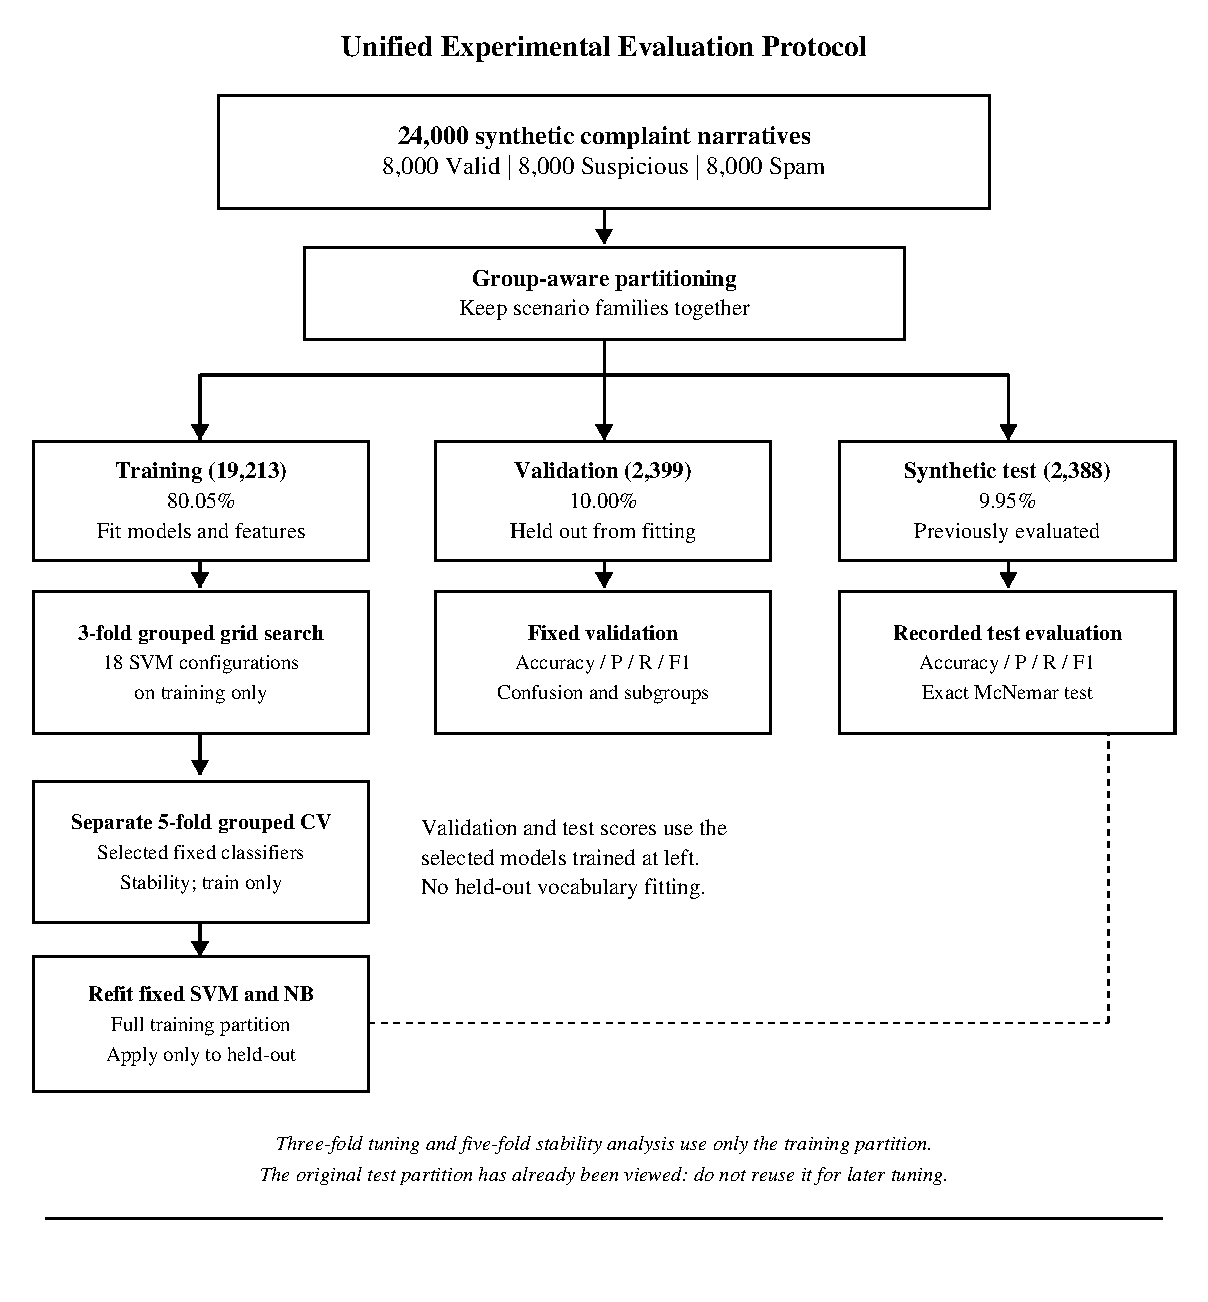
\includegraphics[width=.96\textwidth,height=.80\textheight,keepaspectratio]{figures/m2_unified_evaluation.pdf}\caption{Unified experiment allocation and evaluation protocol. Only the 19,213 training examples participate in model selection and five-fold grouped stability checks; the fixed fitted models are evaluated on 2,399 validation and the previously recorded 2,388 synthetic test examples.}\label{fig:evaluation}\end{figure}

\subsection{Evaluation and Learning Diagnostics}
Accuracy reports the fraction of correct labels, while per-class precision and recall expose specific confusions; Macro-F1 gives equal weight to three classes. Further diagnostics include confusion matrices, class and language subgroup metrics, text-length-only performance, nearest-training-example similarity, and historical challenge summaries. The original challenge input is unavailable for independent re-execution; no replacement challenge is introduced. Learning curves depict accuracy or Macro-F1 as a function of training-set size; these are \emph{not} loss curves over epochs. The final \texttt{LinearSVC} fit does not expose a documented epoch-loss history. Consequently, a separate \texttt{SGDClassifier(loss=hinge)} run recorded epoch-wise training and validation hinge loss. This auxiliary trace supports an optimization discussion but must not be mislabeled as the selected SVM model's own training trace.


\section{Experimental Setup, Reproducibility and Evaluation}
\label{sec:m2}
The recorded experiment used scenario-family-grouped partitioning (19,213 training, 2,399 validation, 2,388 test), three-fold grouped SVM selection over 18 configurations, and a separate five-fold grouped stability analysis. The following sections specify the completed procedures and distinguish them from prospective operational validation.

\subsection{Hardware and Software Environment}\label{sec:environment-final}
Table~\ref{tab:environment-final} distinguishes the documented original research environment from the environment used for subsequent reproducibility verification. Operating-system patches and library versions may differ between executions; both recorded environments are retained for numerical and procedural repeatability.

\begin{table}[H]\centering\caption{Recorded research environment and later verification environment}\label{tab:environment-final}\small\begin{tabularx}{\textwidth}{p{.20\textwidth}XX}\toprule Component & Supplied original record & Later verification record\\\midrule
CPU & Intel Core i7-13700HX & Same CPU model, device query\\
GPU & NVIDIA RTX 4060 Laptop; Intel UHD & Same GPU models, device query\\
RAM & 16 GB; two 8 GB Samsung DDR5-5600 & Two 8 GB Samsung modules at 5600, device query\\
OS & Windows 11 Home 25H2, build 26200.9457 & Windows 11 Home 25H2, build 26200.9711\\
Python & 3.13.5 & 3.13.5\\
scikit-learn & 1.8.0 & 1.8.0\\
NumPy / SciPy & 2.3.5 / 1.17.0 & 2.4.4 / 1.17.1\\
pandas / joblib & 2.2.3 / 1.5.3 & 3.0.2 / 1.5.3\\
Plot/QA dependencies & Not fully captured in original record & Matplotlib 3.11.2; Pillow 12.3.0; threadpoolctl 3.6.0\\\bottomrule\end{tabularx}\end{table}

The actual scikit-learn TF--IDF, LinearSVC and Naive Bayes implementations are CPU-based. No CUDA/GPU estimator or GPU acceleration was used by these scripts; presence of an NVIDIA GPU is an inventory fact. Later verification establishes numerical repeatability of recorded outputs, not bitwise reconstruction of the original environment. The pinned research dependency file represents the verified environment; the supplied historical versions remain identifiable in archival records. Next.js/TypeScript, FastAPI, PostgreSQL and their planned migration/authentication dependencies belong to the proposed application and were not dependencies of the reported offline experiments. pdfLaTeX and the included packages compile the manuscript; their compile logs are artifact evidence, not ML training records.



\subsection{Version Control and Reproducibility}\label{sec:reproducibility-final}
The research repository is \url{https://github.com/rencze/nlp-barangay-complaint-classification-hitl}. Published branch \path{research/milestone2-final-audit}, revision \texttt{17ff46846af10f9554a14ec635390865afba50a3}, identifies the reproducibility package. It contains pinned dependencies, scripts, configurations, saved predictions and models, figures and manuscript source. The canonical input is \path{data/Barangay_Complaint_Dataset_24000.csv}, SHA-256 \path{35414af2dc63e2870928bd1853c557ed301dbdae80416a0bf37be00648d92e28}; stored partitions define the experimental input.

From the repository root, create an isolated Python 3.13 environment, install \path{requirements.txt}, and run \path{python src/minimal_example.py}. This demonstration prints narrative-to-label predictions; it is not a study-performance estimate. \path{python src/verify_dataset.py} checks corpus integrity. Saved evidence is checked by \path{python src/final_evidence_audit.py} and \path{python src/validate_research_artifacts.py}. The original full-study procedures are \path{manuscript/source/reproducibility_scripts/evaluate_models.py} and \path{manuscript/source/validation_suite/run_grouped_validation.py}; exact commands are documented in the repository README. Original outputs must remain preserved when reproducing procedures that write results.

\subsection{Reproducibility Verification and Execution History}\label{sec:verification-history}
The original archived procedures were executed again during the earlier documentation work; logs, environment manifests, historical output copies and recorded-precision comparisons preserve that history. Those executions supported reproducibility, not a new independent study. Historical outputs, subsequent verification outputs and candidate development outputs are separate named artifacts. No dataset was regenerated, relabeled or repartitioned.

Reference model bundles \path{results/verified_20261026/svm_research_only.joblib} and \path{results/verified_20261026/nb_research_only.joblib} contain the matching vectorizer/classifier. \path{src/evaluate_research.py} reloads a trusted bundle for saved-reference evaluation; reference inference passes raw text to that bundle rather than re-fitting vocabulary or applying the demo helper. These research artifact-loading checks are implemented and verified; their integration into authenticated application submission remains planned. Arbitrary uploaded joblib/pickle files must not be loaded. Prediction exports identify records, partitions, labels and model names; immutable artifact SHA-256 manifests and configurations provide lineage. Final figures are regenerated from actual metrics/predictions as 360-DPI PNG and vector PDF/SVG and presented with academic captions/tables, while CSV/JSON remain audit formats.



\subsection{Baseline and Measured Model}
The standard baseline is TF--IDF plus \texttt{MultinomialNB(alpha=1.0)}, a conventional, relatively inexpensive model for sparse text features. The comparison model is word-level TF--IDF plus a linear support vector classifier, \texttt{LinearSVC}. Both are evaluated with identical training, validation and synthetic-test partitions; their target labels are Valid, Suspicious and Spam. The historical scores compare two predeclared text-processing pipelines with the same partition memberships, not estimators operating on exactly equal word features. A fair estimator-only follow-up can use the \emph{same} word n-gram representation in both models, fitted on the existing training partition and assessed through training-group folds and the existing development validation partition. Such a follow-up is not part of the recorded results and must be labeled independently. The separately evaluated concatenated word-plus-character representation is \emph{not} the model whose reported test scores appear in Chapter~4.

\subsection{Evaluation Metrics and Error Analysis}\label{sec:metrics-final}
Let $K=3$ classes, $N$ evaluated narratives, $y_i$ the reference text label of record $i$, and $\hat y_i$ its prediction. For class $c$, $TP_c$ counts correctly predicted class-$c$ records, $FP_c$ counts other-class records predicted as $c$, $FN_c$ counts class-$c$ records predicted otherwise, and $TN_c$ counts records neither reference nor predicted as $c$. Let $n_c$ be reference support in class $c$ and $\mathbf{1}[A]$ equal one when condition $A$ is true, otherwise zero. For single-label multiclass classification:
\begin{align}
\mathrm{Accuracy}&=\frac{1}{N}\sum_{i=1}^{N}\mathbf{1}[y_i=\hat y_i]=\frac{\sum_{c=1}^{K}TP_c}{N},\\
P_c&=\frac{TP_c}{TP_c+FP_c}, & R_c&=\frac{TP_c}{TP_c+FN_c},\\
F_{1,c}&=\frac{2P_cR_c}{P_c+R_c}=\frac{2TP_c}{2TP_c+FP_c+FN_c},\\
P_{\mathrm{macro}}&=\frac{1}{K}\sum_c P_c,&R_{\mathrm{macro}}&=\frac{1}{K}\sum_c R_c,\\
F_{1,\mathrm{macro}}&=\frac{1}{K}\sum_c F_{1,c},&F_{1,\mathrm{weighted}}&=\frac{1}{N}\sum_c n_cF_{1,c}.
\end{align}
Zero-denominator class scores are set to zero explicitly. Accuracy expresses overall agreement; precision describes how often predictions of a class are correct; recall describes how many reference examples of that class are recovered. F1 balances precision and recall. Macro-F1 is the primary measure because it gives each of the three operational text labels equal influence rather than letting a common class dominate. Weighted-F1 reflects reference support. Macro-F1 is the mean of class F1 scores, not the F1 of macro-precision and macro-recall.

The confusion entry $M_{ab}=\sum_i\mathbf{1}[y_i=a\land\hat y_i=b]$ counts reference class $a$ predicted as class $b$; rows are reference labels and columns are predictions. Per-class precision/recall/F1/support, mistakes, language-group support and confusion counts accompany aggregate metrics in Chapter~4. A Valid narrative predicted as Spam is particularly important because inappropriate rejection or deprioritization could prevent access to assistance. The proposed routing therefore sends Spam to human review rather than rejecting it automatically. Label agreement neither verifies an incident's factual truth nor measures complaint-resolution effectiveness.

Training-size learning curves measure Macro-F1 as sample count changes. \texttt{LinearSVC} does not emit the reported epoch-loss history; the fifteen-pass SGD hinge-loss trace is a distinct auxiliary estimator and must remain labeled accordingly. Length-only and character-only ablations are diagnostic checks for generator shortcuts rather than deployed alternatives. The reported word/character candidate is separately described below.



\subsection{Actual Hyperparameter Search and Selection}
The recorded SVM search used \texttt{GridSearchCV} with three-fold, scenario-family-grouped cross-validation on the 19,213 training records. It examined 18 combinations (three $C$ values by two word-ngram choices by three minimum-document-frequency values); all learned TF--IDF statistics were fitted within training folds. The later, separate five-fold \texttt{StratifiedGroupKFold} experiment retested the selected settings for stability; it did not perform the original search again.
\begin{table}[H]\centering\caption{Recorded fixed and varied hyperparameter settings}\label{tab:m2grid}\small\begin{tabularx}{\textwidth}{p{.39\textwidth}X}\toprule
Setting & Recorded value(s)\\\midrule
\texttt{LinearSVC.C} (variable) & $\{0.1,1,10\}$\\
\texttt{TfidfVectorizer.ngram\_range} (variable) & $\{(1,1),(1,2)\}$ (word analyzer)\\
\texttt{TfidfVectorizer.min\_df} (variable) & $\{2,5,10\}$\\
\texttt{max\_df} / \texttt{sublinear\_tf} (fixed) & $0.95$ / enabled\\
Primary tuning metric & Grouped three-fold mean Macro-F1\\
Selection from tied candidate scores & $C=0.1$, word unigrams, \texttt{min\_df}=2 (deterministic tie handling)\\
Follow-up stability analysis & Separate five-fold grouped CV on training partition\\
Random seed & \texttt{20261026}\\\bottomrule
\end{tabularx}\end{table}
The grouped grid is selected by mean Macro-F1 with deterministic tie handling; observed scores and their interpretation are reported in Chapter~4. The reserved evaluation records were not used to fit TF--IDF or select this grid. The unified allocation and validation protocol is summarized in Figure~\ref{fig:evaluation}.

\subsection{Statistical Model Comparison}
Because the SVM and Naive Bayes predict the \emph{same} held-out narratives, their correct-versus-incorrect outcomes form paired binary observations. McNemar's test is therefore appropriate for comparing error occurrence between \emph{two} classifiers on a common test partition \cite{mcnemar_nist}. Let $b$ be the count correctly classified by the baseline but wrongly by SVM, and $c$ the count wrongly classified by the baseline but correctly by SVM. The continuity-corrected large-sample statistic and the small-discordance exact alternative are:
\begin{align}
\chi^2_{\mathrm{McN}} &= \frac{\max(0,|b-c|-1)^2}{b+c},\quad b+c>0,\\
X&\sim\mathrm{Binomial}(b+c,\tfrac12),\quad
p_{\mathrm{exact}}=\min\!\left\{1,2\Pr\big[X\leq\min(b,c)\big]\right\}.
\end{align}
The hypothesis $H_0$ is equal paired error probabilities, tested at $\alpha=0.05$. The exact binomial form is preferred for the present experiment's small number of discordant pairs. Actual paired predictions, contingency counts and interpretations are reported in Chapter~4. The repeated historical test is not a new independent test. A Friedman test would concern a different design involving more classifiers and repeated comparable datasets; it is not justified by the current two-model, one-test-set comparison.

\subsection{Model Evaluation Sequence}
The actual reproducible sequence is (1) preserve the 24,000-row synthetic source, codebook and scenario-group IDs; (2) group-partition into 19,213/2,399/2,388; (3) fit the baseline and perform three-fold grouped SVM grid search on training only; (4) conduct a separate five-fold grouped stability analysis on the training portion; (5) evaluate the selected fixed models on 2,399 validation records and the previously evaluated 2,388 synthetic test records; (6) report class-wise and aggregate scores, confusion matrices and exact paired-error comparison; and (7) document scripts, seed, versions, selected parameters, generator limitations and the limitation that performance outside this synthetic corpus is not measured. Chapter~4 contains \emph{observed results}; combined features and calibration are separately evaluated development candidates, while operational HITL and model retraining remain proposed system capabilities.

\section{Reproducibility Protocol and Evidence Boundary}
\label{sec:prerun}
For the completed rerun, the researchers preserved the supplied \texttt{ALL\_SYNTHETIC\_V2.csv} and its recorded partition memberships. \textbf{The current repeatability exercise uses the same 24,000-record synthetic corpus; no additional dataset or relabeling is part of this reproduction.} The set comprises 19,213 rows for fitting and grouped cross-validation, 2,399 rows for fixed development validation, and 2,388 rows for the historically evaluated synthetic test. Only the training partition is used for estimator and TF--IDF fitting. A validation score is not a training score, and a repeated score from the same test rows is not new external evidence.

The GitHub artifact should record a Git commit identifier, the SHA-256 of the 24,000-row source file, Python and library versions, experiment seeds and exact commands. The dataset partitions are exported from the \texttt{split} column without generating or resampling records, and a preflight script checks disjoint scenario-family IDs and counts before model fitting. The two principal reproducible commands are \path{python reproducibility_scripts/evaluate_models.py} for the original model comparison and \path{python validation_suite/run_grouped_validation.py} for the separate five-fold training-only stability audit. The repository also includes a small smoke test, which is not evidence of full-study accuracy. Since the full scripts may overwrite recorded outputs, the original result files must be archived and versioned before a rerun. Any discrepancy is logged, not silently rewritten into the thesis.

Reproducibility verification established whether the recorded preprocessing, SVM, Naive Bayes and cross-validation scripts execute on unchanged splits. If a second, explicitly labeled \emph{sensitivity experiment} compares a common TF--IDF representation or the proposed word--character combination, it must use training-group folds and the existing development validation partition for configuration decisions. It must not use the previously viewed synthetic test as an unseen selection set. Report the new settings and results separately instead of replacing the historical scores. A subsequent combined-feature/calibration experiment was executed on development validation only; operational HITL, feedback retraining and live case management remain untested regardless of their appearance in design diagrams.

\subsection{Reproducibility Artifacts}
\begin{table}[H]\centering\caption{Reproducibility artifacts and what each establishes}\label{tab:preruncheck}\small
\begin{tabularx}{\textwidth}{p{.34\textwidth}X}\toprule
Artifact & Required evidence \\\midrule
Source CSV and split files & Source hash; partition totals; label counts; no scenario-family overlap across partitions. \\
Baseline and SVM scripts & Refit TF--IDF within each training fold; record selected parameters and seeds. \\
Validation metrics & Accuracy, class-wise precision, recall, F1, Macro-F1, weighted-F1 and confusion matrices on 2,399 records. \\
Synthetic test archive & Historical scores on 2,388 records, explicitly marked as already evaluated; preserve paired predictions if available. \\
Five-fold stability audit & Training-only grouped folds; group overlap report and fold-wise metrics. \\
README, environment and commit & Installation instructions, exact commands, dependency versions and source-code revision. \\\bottomrule
\end{tabularx}\end{table}

\section{Required Next Validation Protocol}
As \emph{future validation recommendations}, rather than conditions claimed to have been completed in the current single-corpus rerun, robust deployment evaluation would include: (a) independent blinded human label agreement; (b) broader unseen-scenario / root-seed holdout independent of template families; (c) deliberately constructed minimal-pair tests of ambiguous versus clear narratives; (d) subgroup performance on Bisaya, Filipino, English and mixed inputs; (e) safety-sensitive false-negative review; (f) probability/margin reliability and an abstention or ``review required'' policy; and (g) full-stack end-to-end tests for accounts, audit logs, urgency escalation, status transitions, feedback consent, versioning, latency and rollback. These items are not evidence generated by the current experiment. The immediate documented rerun uses only the existing synthetic corpus and its stored train/validation/test membership; any subsequent external assessment, if undertaken, must be reported as a separate study.

\section{System Architecture and Operational Boundary}
The proposed system distinguishes a researcher-evaluated word-level TF--IDF/SVM baseline from a planned operational architecture that adds privacy-aware input preparation, class-based HITL review, accepted-case management and controlled retraining. Word-plus-character features and sigmoid calibration were separately evaluated on synthetic development validation; they do not establish operational reliability. The measured model scores are not evidence that the additional production functions are already implemented or validated. Section~\ref{sec:proposed-operational-workflows} defines these interfaces, states and non-automatic feedback processes. System-level monitoring and administrator accountability are application requirements to be evaluated separately from classifier accuracy.


\label{sec:proposed-operational-workflows}
\textbf{Implementation boundary.} Figures in this section specify the \emph{target application design}. They are not additional completed experiments. The reproducible results in this manuscript concern the existing synthetic-data word-level TF--IDF and Linear SVM pipeline. The combined word/character representation and grouped sigmoid calibration were separately tested on existing synthetic development validation. Live probability reliability, class-dependent administrative review, case management and feedback-driven retraining still require independent implementation and measurement before production-readiness claims. Each diagram is placed immediately after the explanatory discussion of its named process; figure numbers are assigned by LaTeX captions rather than embedded in the graphics.

\subsection{Complaint Intake and Input Boundary}
The proposed resident-side form requires a \emph{Subject} and a \emph{Complaint Narrative}. If known, a date/time of occurrence and an approximate Purok/Sitio or landmark can be supplied as supporting context, without compulsory GPS or an interactive map. The narrative, not the user's name, phone number, assigned language tag or other metadata, is the primary input to the three-class SVM. The subject can be retained for case identification, but adding it to the classifier requires a separately documented experiment to preserve comparison with the recorded text-only baseline. The application should provide a confirmation and tracking reference and maintain authenticated access and lawful handling of resident information. The screenshots of Davao City Reports serve as a \emph{local interface precedent}, not evidence that its implementation has been replicated \cite{dcr,ra10173}.

The core scope excludes photo uploads, image classification, ensembles that combine images and text, automated determination of physical truth and mandatory GPS coordinates. Where urgent safety reports arise, an independent referral/escalation safeguard is recommended rather than allowing an ordinary three-class text prediction to prevent timely review. Such referral logic remains a system requirement, not an experimentally demonstrated function.

\subsection{NLP Preprocessing: Meaning-Preserving Candidate}
Figure~\ref{fig:op-nlp} specifies a proposed conservative NLP routine. A secure original can be retained for authorized processing while the model operates on a minimized copy with direct identifiers masked when appropriate. The depicted privacy-oriented operational routine uses Unicode NFC, whitespace normalization, lowercasing and limited cleanup; these are intended to standardize representation without discarding \emph{hindi}, \emph{wala}, \emph{no}, \emph{not}, relevant number expressions or incident descriptions. Generic stopword removal, stemming and lemmatization are excluded from this proposed routine to avoid meaning-altering changes to mixed-language complaints. The current reproducibility scripts use scikit-learn TF--IDF's text processing; the separately depicted privacy masking and normalization stages are not asserted to be fully implemented in those recorded experiments. The separately evaluated development candidate instead uses NFKC/casefold/whitespace and no identifier masking, as specified in Section~\ref{sec:candidate-final}; these preprocessing variants must not be interchanged silently. Any masking accuracy must be assessed because over-masking can remove useful context and under-masking can expose personal information \cite{ra10173,sklearnpitfalls}.
\begin{figure}[H]\centering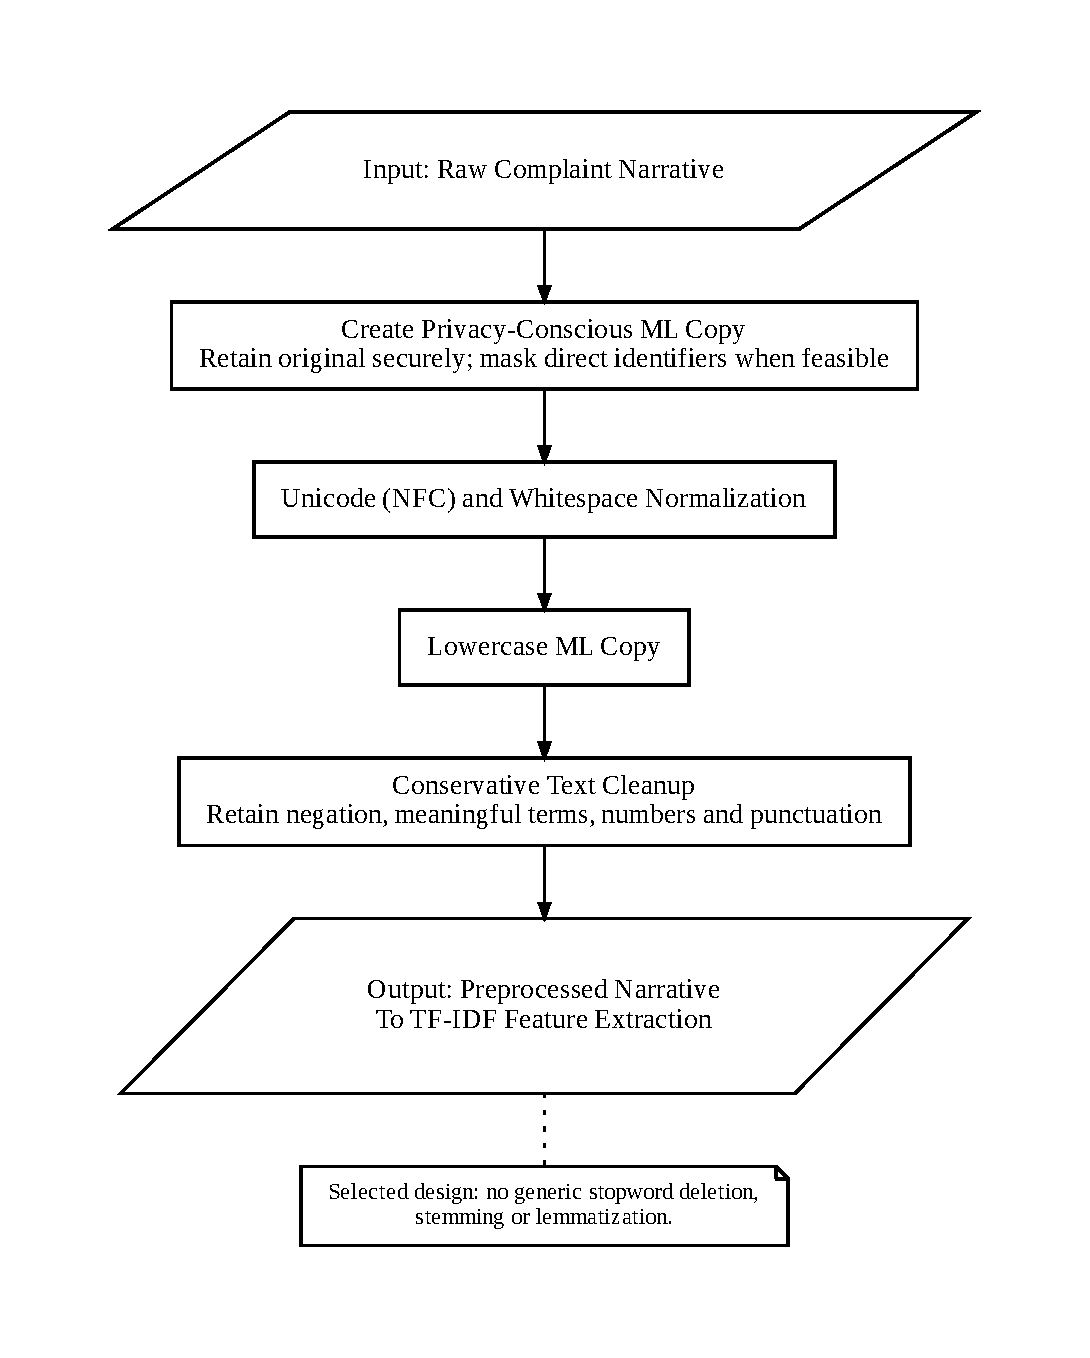
\includegraphics[width=.94\textwidth,height=.69\textheight,keepaspectratio]{figures/nlp_proposed.pdf}\caption{Proposed Natural Language Processing (NLP) preprocessing workflow for complaint narratives. Privacy-aware masking and normalization are target features, not measured preprocessing steps in the reported synthetic-data experiments.}\label{fig:op-nlp}\end{figure}

\subsection{TF--IDF Feature Extraction and Model-Level Consistency}
The recorded main SVM results used word-unigram TF--IDF, with a separately examined character-only ablation. Figure~\ref{fig:op-tfidf} describes the separately evaluated candidate using word unigrams and bigrams \emph{together with} character-within-word 3--5-grams. The resulting two sparse feature matrices are concatenated before classification. This combination is a \emph{separately evaluated development candidate}, not the verified configuration yielding the previously reported perfect within-generator score. In both configurations, vocabulary and inverse-document-frequency weights must be fitted within training partitions, never independently refitted on each new complaint. The deployed vectorizer and classifier should be versioned together \cite{sklearntfidf,sklearnpitfalls}.
\begin{figure}[H]\centering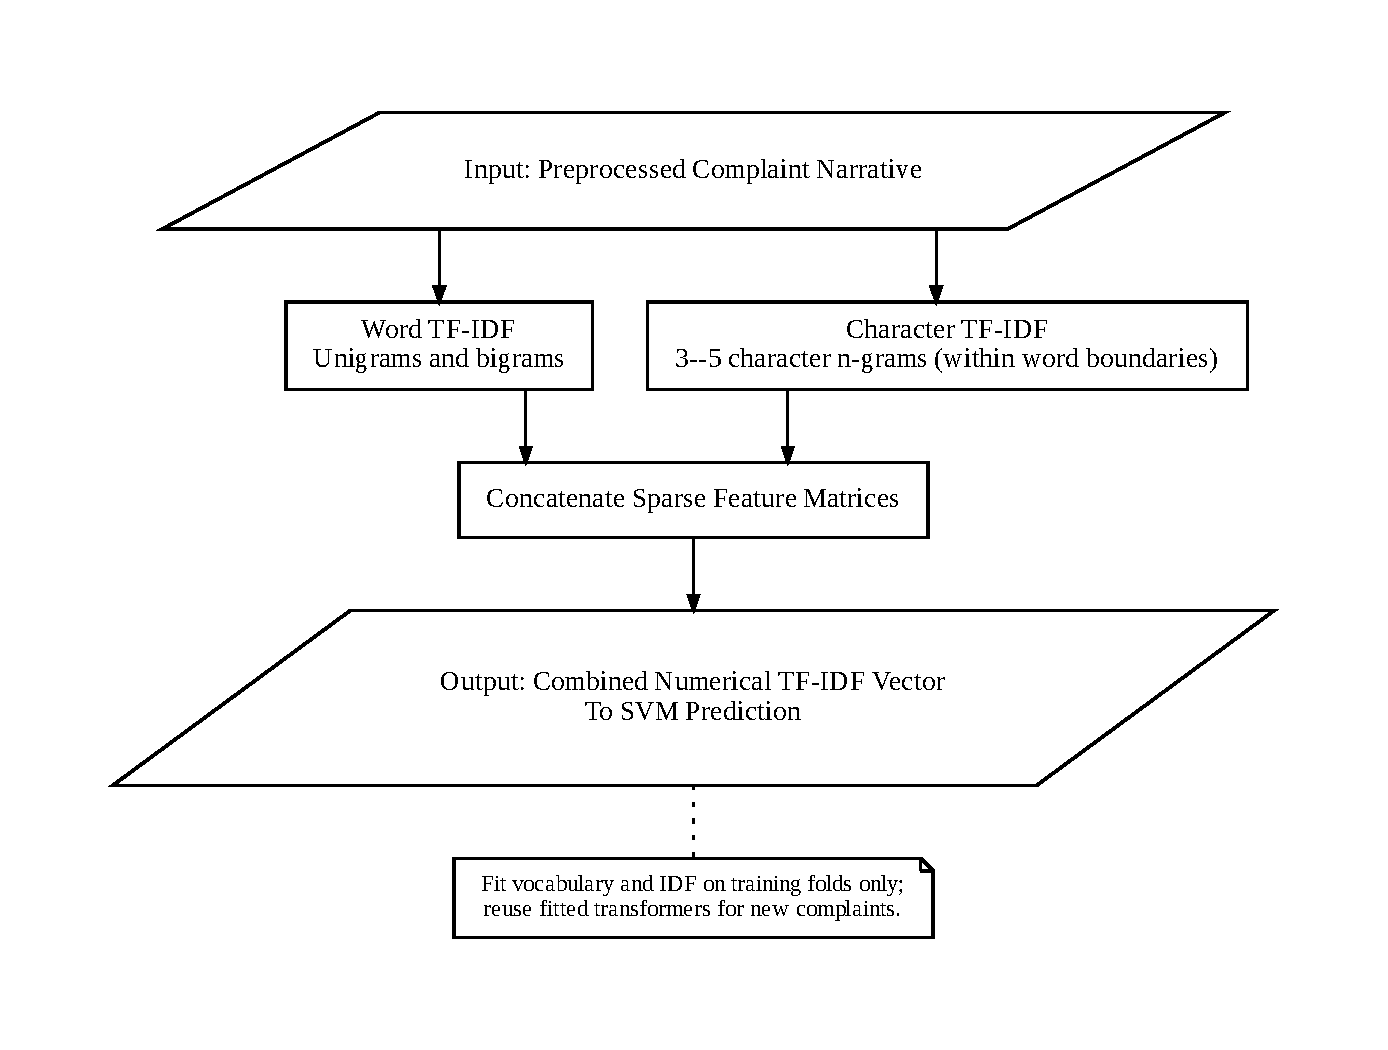
\includegraphics[width=.96\textwidth,height=.68\textheight,keepaspectratio]{figures/tfidf_proposed.pdf}\caption{Separately evaluated word--character TF--IDF candidate. Concatenation and grouped sigmoid calibration were evaluated on development validation and tied the original word-only SVM Macro-F1; operational deployment and external reliability remain unvalidated.}\label{fig:op-tfidf}\end{figure}

\subsection{SVM Training and Calibrated Prediction}
Figure~\ref{fig:op-svm} separates model fitting from inference. An offline Linear SVM is trained using authorized labeled data, with hyperparameter selection performed through training-only cross-validation. Before model probabilities can be described as \emph{calibrated}, an appropriate calibrator must be fitted using independent calibration folds or held-out training material, then evaluated for reliability. During inference, a new complaint is transformed by the saved compatible vectorizer and classified by the saved model; it is not used to fit the model. The three displayed class-probability quantities remain proposed operational outputs; the reference SVM is uncalibrated, while a separate candidate supplies synthetic development probability diagnostics in Chapter~4 \cite{sklearncalib,sklearnpitfalls}.
\begin{figure}[H]\centering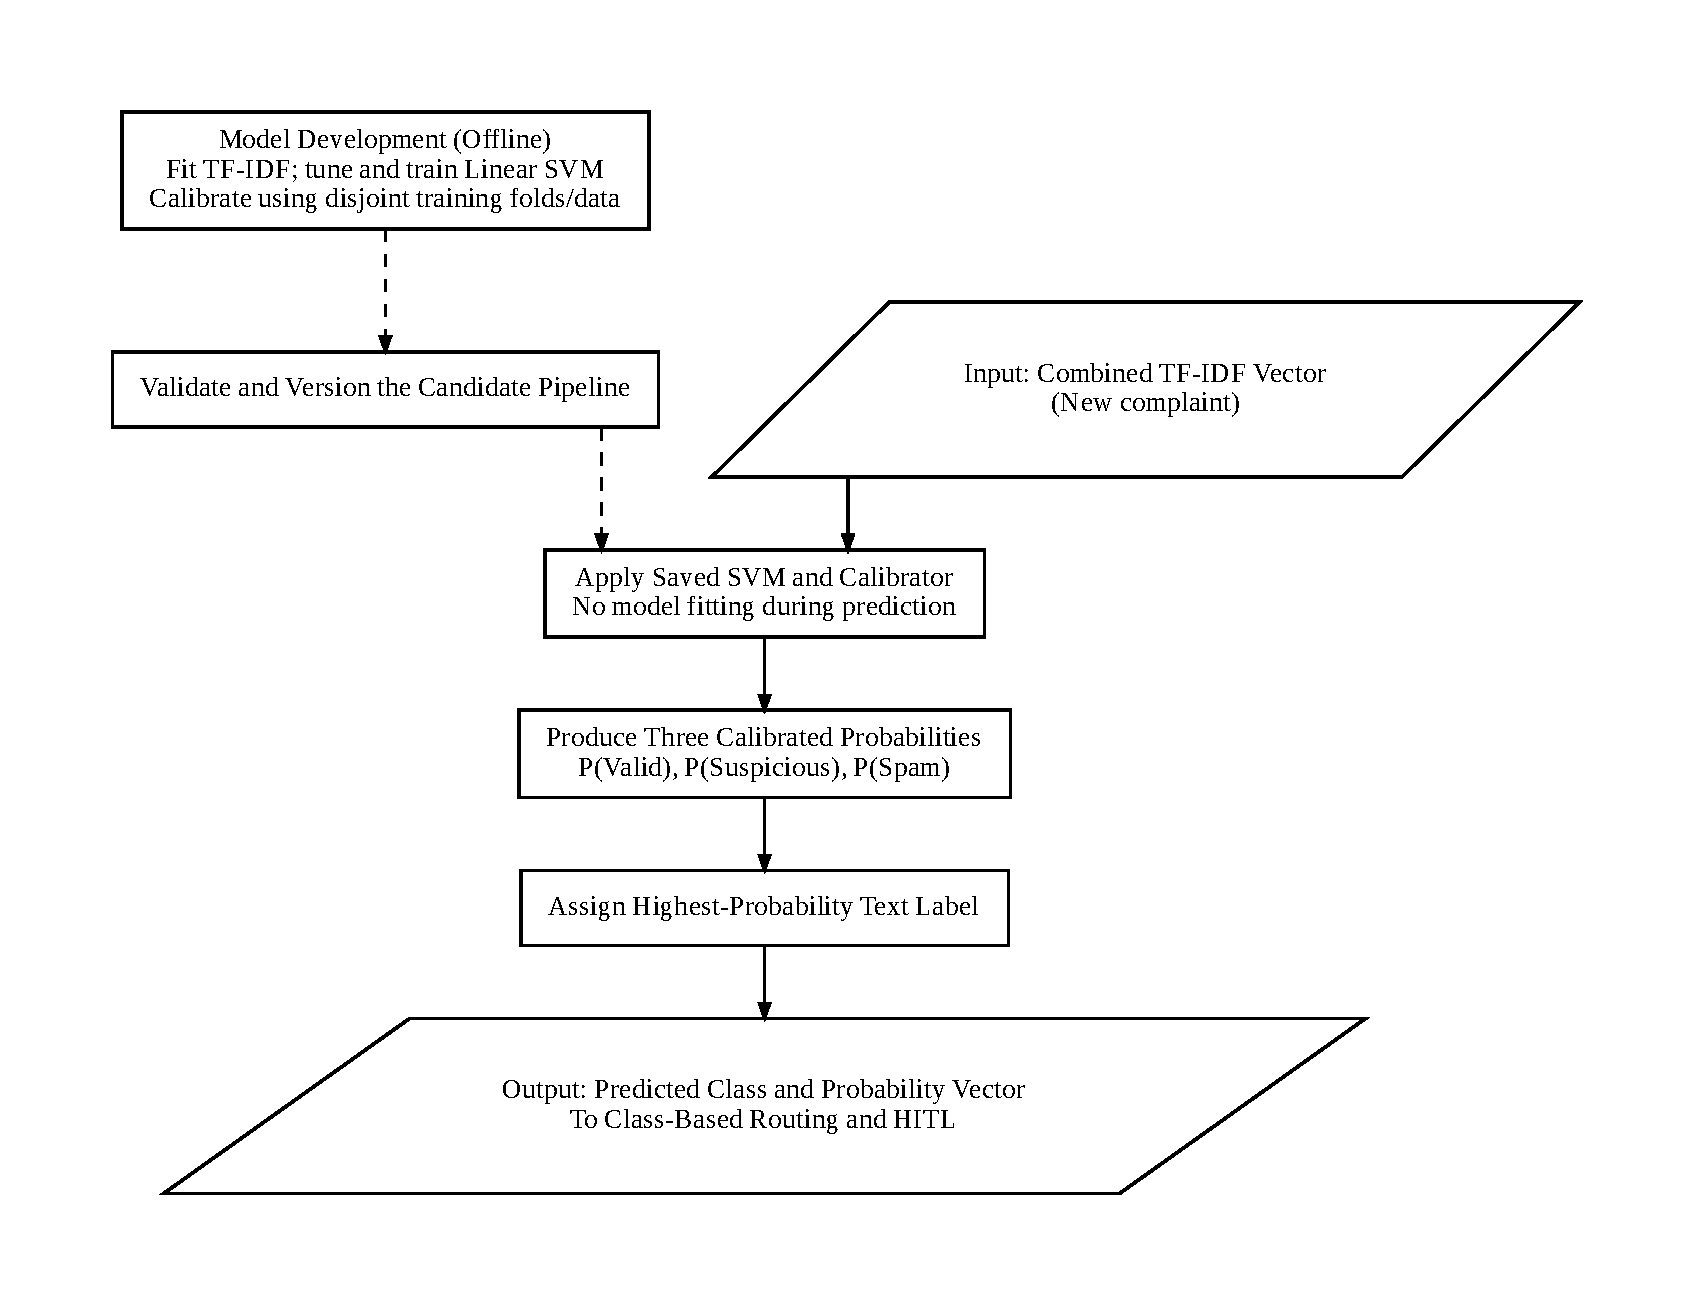
\includegraphics[width=.96\textwidth,height=.72\textheight,keepaspectratio]{figures/svm_proposed.pdf}\caption{Proposed support vector machine (SVM) model-development and new-complaint prediction workflow, with a separate probability-calibration requirement.}\label{fig:op-svm}\end{figure}

\subsection{Human-in-the-Loop Verification and Administrative Disposition}
The initial proposed routing rule is \emph{class-based}: predictions of Valid go directly to accepted-case handling, while predicted Suspicious or Spam are referred to the administrator for Human-in-the-Loop (HITL) review. Calibrated scores, once validated, may help \emph{prioritize} cases within the review queue; no numerical cutoff is fixed by this study. Under this design, an error that predicts Valid will not enter routine HITL, so a separately selected random audit of predicted Valid cases is necessary to estimate unobserved misclassifications. This is a proposed mitigation of the selective-label problem, not an implemented audit \cite{lakkaraju2017,madras2018}.

The administrator first examines the particular original text version and may confirm or correct its \emph{text label} to Valid, Suspicious or Spam. Separately, the administrator makes the \emph{disposition}: Accepted, Pending Clarification or Rejected with documented reason. Figure~\ref{fig:op-hitl} shows the decision boundary. A predicted Spam that was actually a clear complaint can be corrected to Valid and accepted; an incomplete original can remain Suspicious while external clarification permits administrative acceptance. No accepted case is automatically converted to a Valid training label, and no rejected case is automatically converted to Spam. A clarification request must be reassessed after a response or the applicable policy-governed response period; no invented universal deadline is imposed \cite{rottger2022,fleisig2024,franc2023}.
\begin{figure}[H]\centering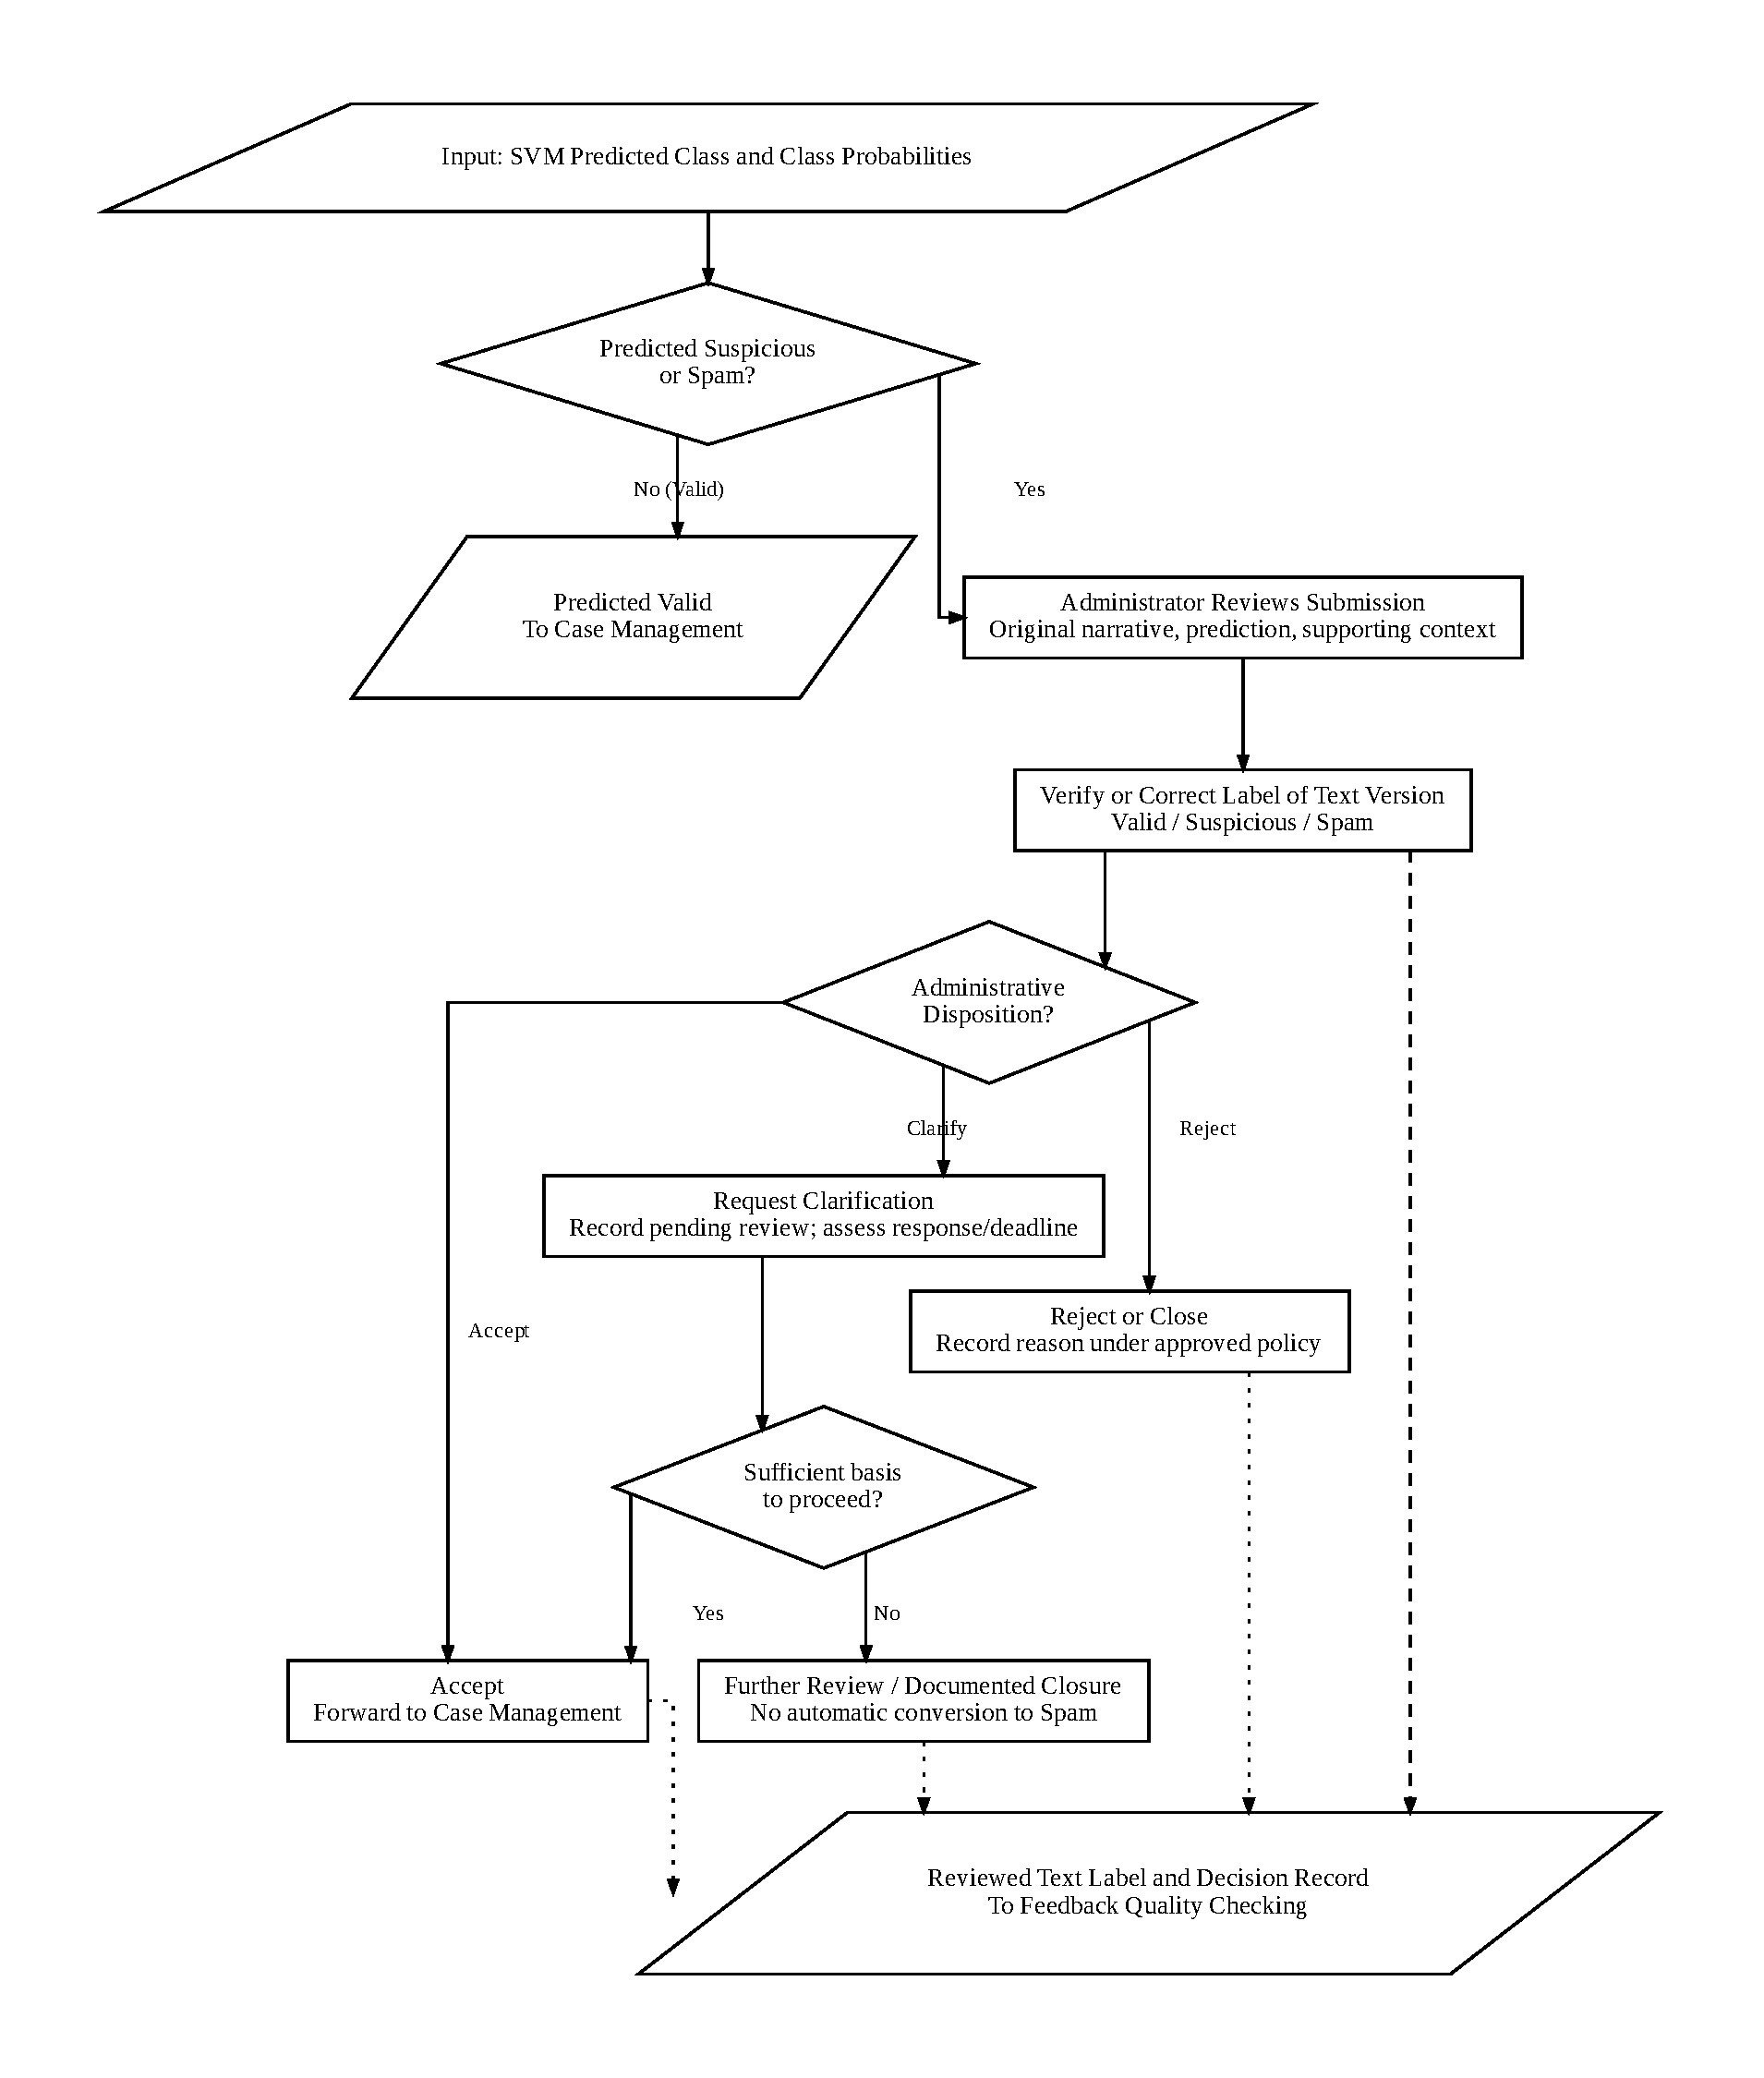
\includegraphics[width=.96\textwidth,height=.83\textheight,keepaspectratio]{figures/hitl_proposed.pdf}\caption{Proposed Human-in-the-Loop complaint review with distinct text-label verification and administrative disposition. Only predicted Suspicious or Spam enter routine HITL; direct Valid predictions proceed separately.}\label{fig:op-hitl}\end{figure}

\subsection{Nine Boundary Scenarios for Consistent Labeling}
Table~\ref{tab:op-boundary} operationalizes the ambiguous cases found in the consolidated evidence review. The text label applies to the \emph{narrative version}, not the independently investigated incident or the administrative case outcome. These are annotation and workflow rules to be validated by reviewers, not performance findings from an authentic dataset \cite{rottger2022,fleisig2024,li2023}.
\begin{longtable}{p{.39\textwidth}p{.23\textwidth}p{.29\textwidth}}
\caption{Proposed boundary-case labeling and administrative handling rules}\label{tab:op-boundary}\\
\toprule Scenario & Verified narrative label & Administrative handling\\\midrule\endfirsthead
\toprule Scenario & Verified narrative label & Administrative handling\\\midrule\endhead
Predicted Suspicious, but original text is already clear. & Correct to Valid. & Accept and route to case management.\\
Original is vague; resident supplies complete revision. & Original Suspicious; revised Valid. & Accept revised narrative; preserve both versions.\\
Original vague; independent evidence supports proceeding. & Original remains Suspicious. & May accept if authorized procedure permits.\\
Predicted Spam, but original is an actionable complaint. & Correct to Valid. & Accept; do not automatically reject.\\
Predicted Spam, but original is complaint-related and incomplete. & Correct to Suspicious. & Clarify; accept if sufficient information follows.\\
Predicted Suspicious, but content is promotional non-complaint material. & Correct to Spam. & Reject after human confirmation and record reason.\\
Text is clear but allegation has not been substantiated. & Valid as text. & Investigate or document outcome; truth not inferred by SVM.\\
Clear text later has legitimate administrative grounds for closure or rejection. & Valid as text. & Record grounds without changing text label.\\
Repeated similar submissions from one or several residents. & Label each version by its text. & Check duplicates and corroboration independently.\\
\bottomrule\end{longtable}

\subsection{Verified Feedback, Data Quality and Controlled Model Retraining}
Figure~\ref{fig:op-retrain} begins with versioned human-reviewed label records; it does not repeat the administrative Accept/Reject workflow. Records first undergo quality, duplicate, provenance, privacy and split-family checks. They are then accumulated in a verified-feedback pool. A periodic review of count, verified-class distribution, diversity, repeated errors and performance degradation determines whether a candidate training run is justified; the run requires authorization. Retraining is \emph{not triggered by each click} on an administrative button. An approved run consolidates the existing eligible training material and the new verified examples, refits the preprocessing and vectorization components, trains and recalibrates a candidate SVM, and evaluates it on a fixed independent validation protocol. A candidate that fails release criteria is archived without replacing the live model; a candidate that passes can be separately approved and versioned for future predictions \cite{figueroa2012,ghose2024,sklearnpitfalls,nist}.

The consolidated research review proposes cumulative increments of \emph{100, 250 and 500} verified examples as learning-curve checkpoints, with 1,000 only if feasible. They are \emph{research planning choices}, not empirically validated minimums or automatic deployment triggers. The baseline plus those three candidates are four conceptual model configurations, but cross-validation and calibration can require many additional fits. All variants of one case and related synthetic templates must remain grouped to prevent evaluation leakage. A small independent audit of predicted Valid cases should prevent the feedback pool from consisting solely of Suspicious/Spam predictions. Existing synthetic-data Macro-F1 scores cannot demonstrate that retraining on authentic complaints improves generalization \cite{figueroa2012,beatty2018,citovsky2021,ghose2024,lakkaraju2017}.
\begin{figure}[H]\centering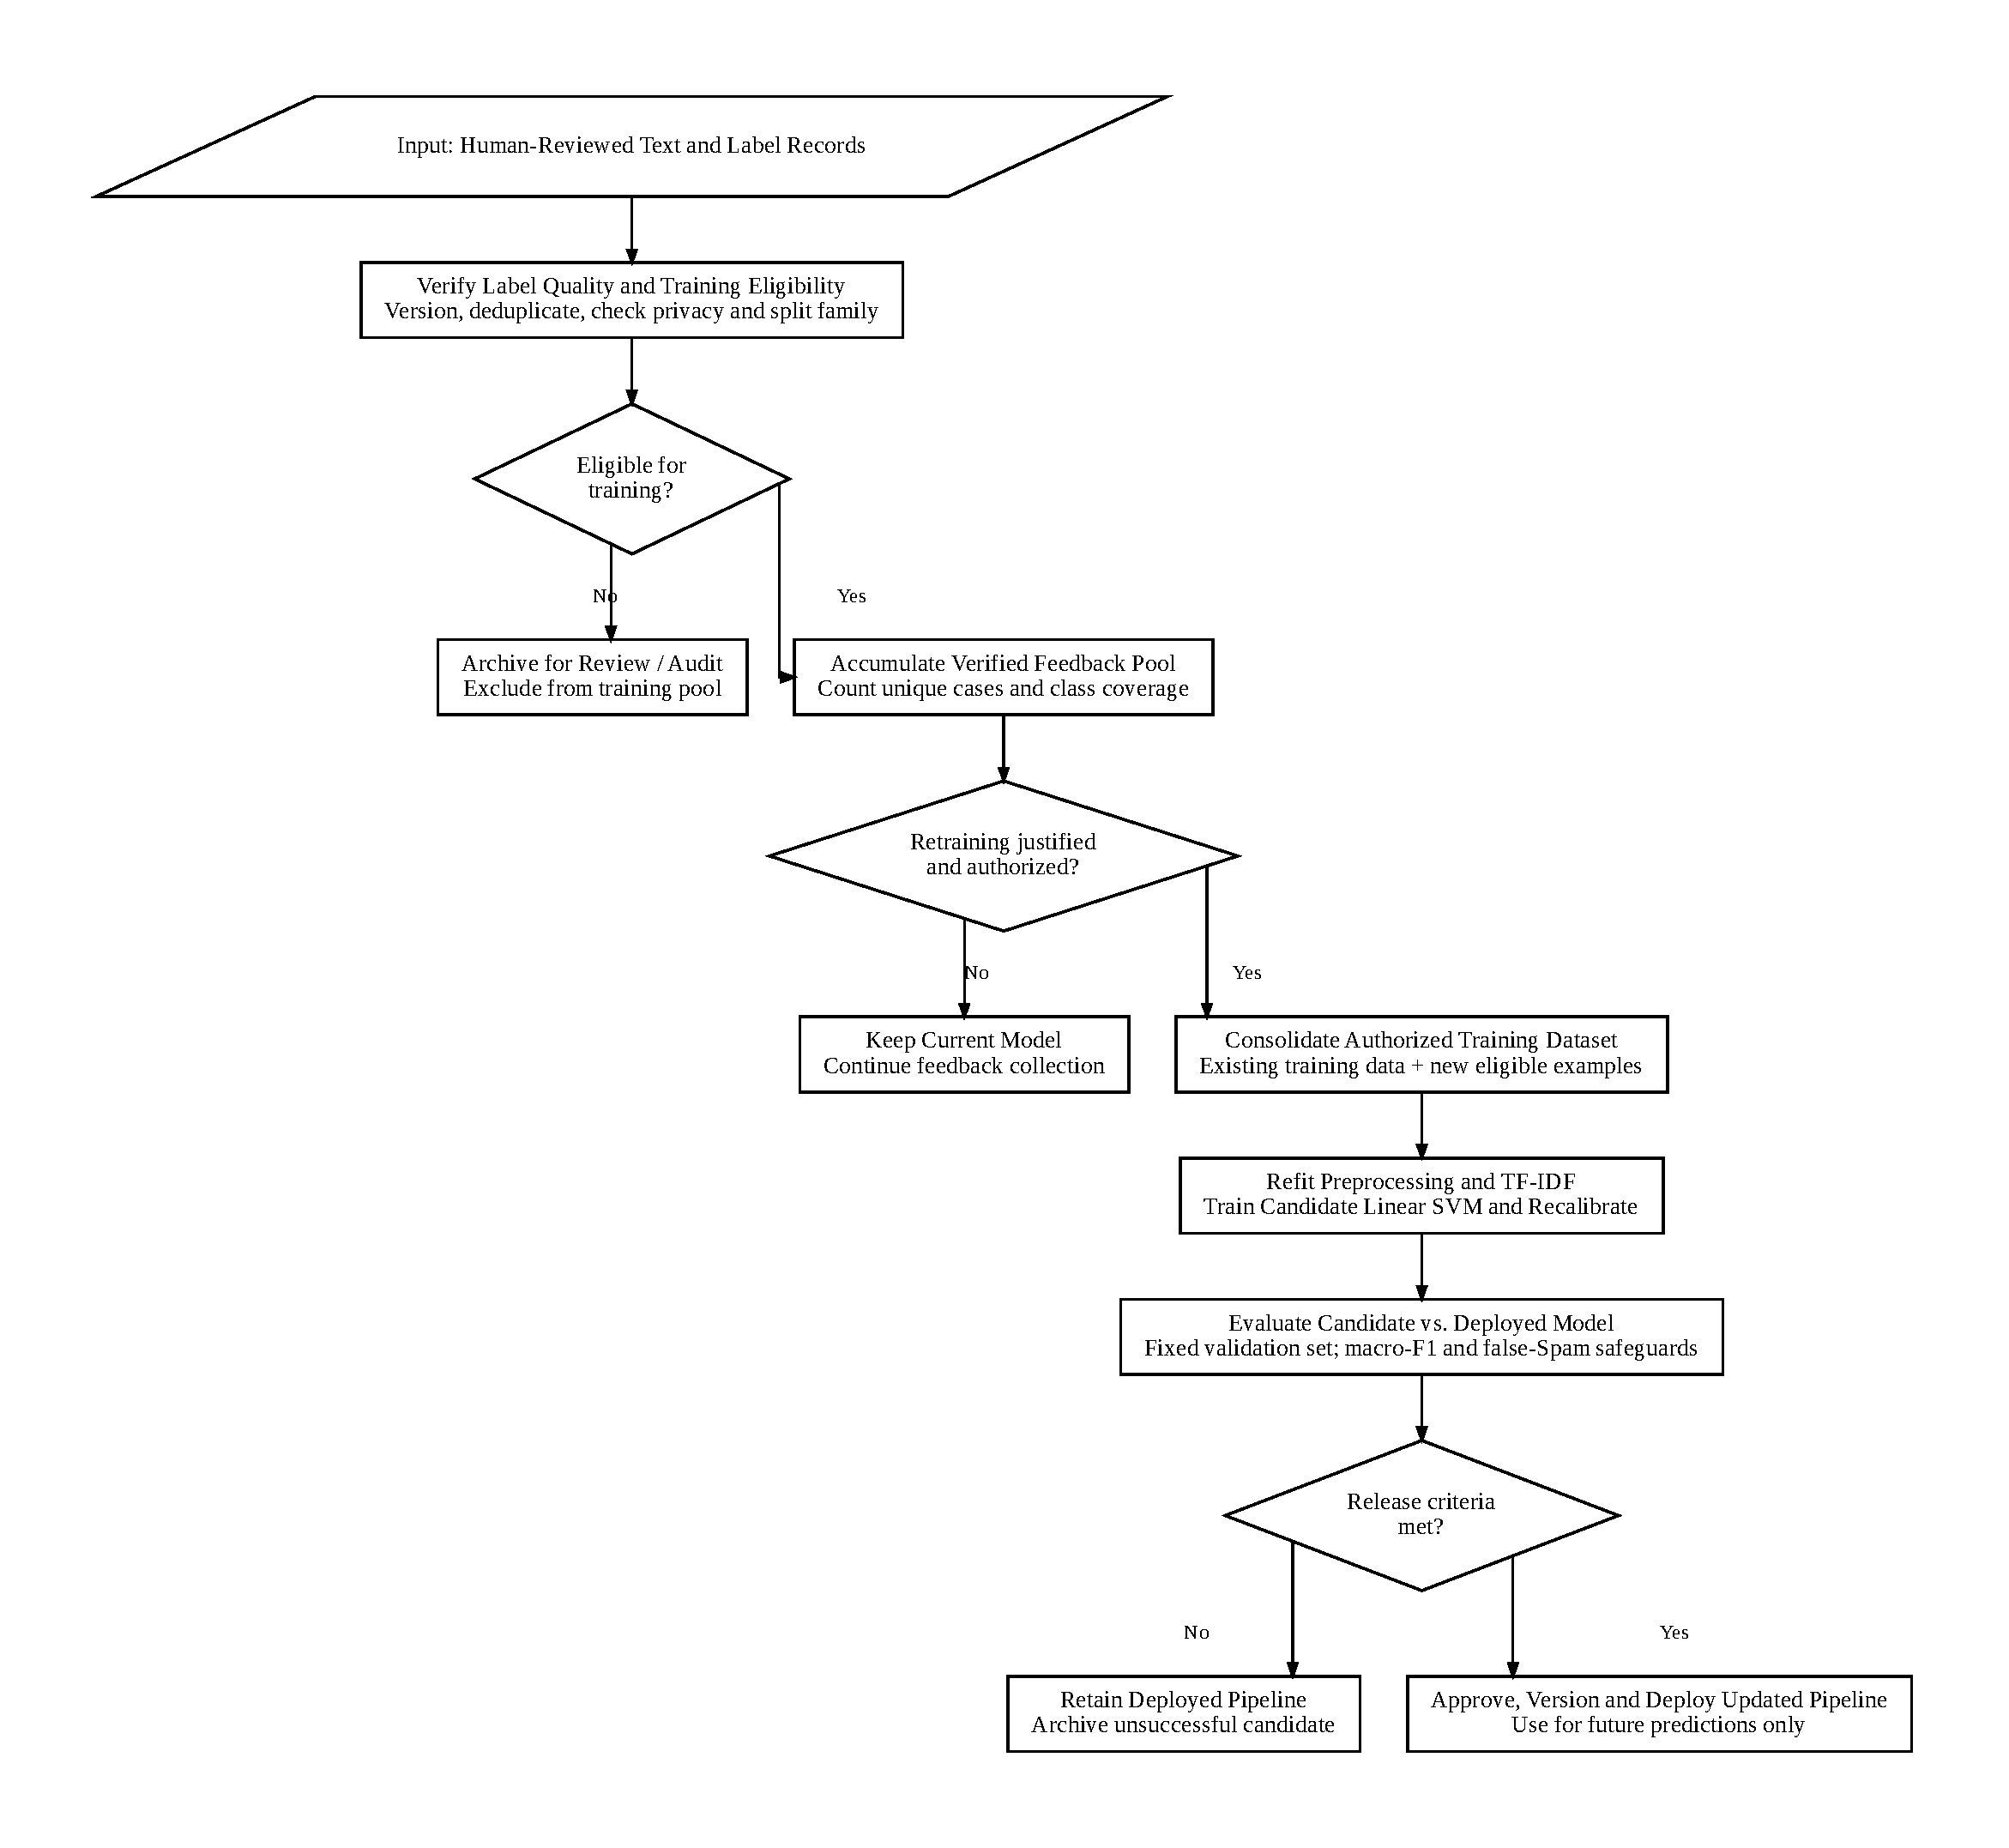
\includegraphics[width=.96\textwidth,height=.83\textheight,keepaspectratio]{figures/retrain_proposed.pdf}\caption{Proposed quality-checked human feedback and controlled batch retraining; training eligibility and deployment approval are separate decisions, and failure does not trigger infinite retries.}\label{fig:op-retrain}\end{figure}

\subsection{Accountable Complaint Case Management (Accepted Cases Only)}
The accepted-case workflow in Figure~\ref{fig:op-case} begins after the system accepts a predicted Valid narrative or an authorized administrator accepts a reviewed submission. The case receives a tracking identifier and a principal state of \emph{Unresolved}; designation of responsible staff, documented investigation and progress updates move the case to \emph{Ongoing}; independently checked completion allows it to become \emph{Resolved}. Records capture officer assignment, action timestamps, correspondence and supporting justification. \emph{Overdue}, \emph{Referred} and \emph{Reopened} are auditable events or flags, not additional SVM labels. If an action is unfinished, disputed or inadequately verified, the case returns to follow-up rather than being silently finalized.

This proposed administrative design is grounded in the distinction between public \emph{response obligations} and full incident resolution. Republic Act No.~6713, Section~5(a), addresses replies to public communications within fifteen working days; Republic Act No.~11032 and the relevant Citizen's Charter govern processing of covered services by complexity. The special 72-hour concrete-action standard associated with the national 8888 channel is \emph{not} a universal deadline for resolving every barangay incident. The application must store the locally applicable rule, permit reasoned referral/escalation and support resident disagreement. Davao City Reports provides a local precedent for tracking references, progress history and re-filing, not a claim that this proposed barangay implementation already meets its requirements \cite{ra6713,ra11032,eo8888,dcr}.
\begin{figure}[H]\centering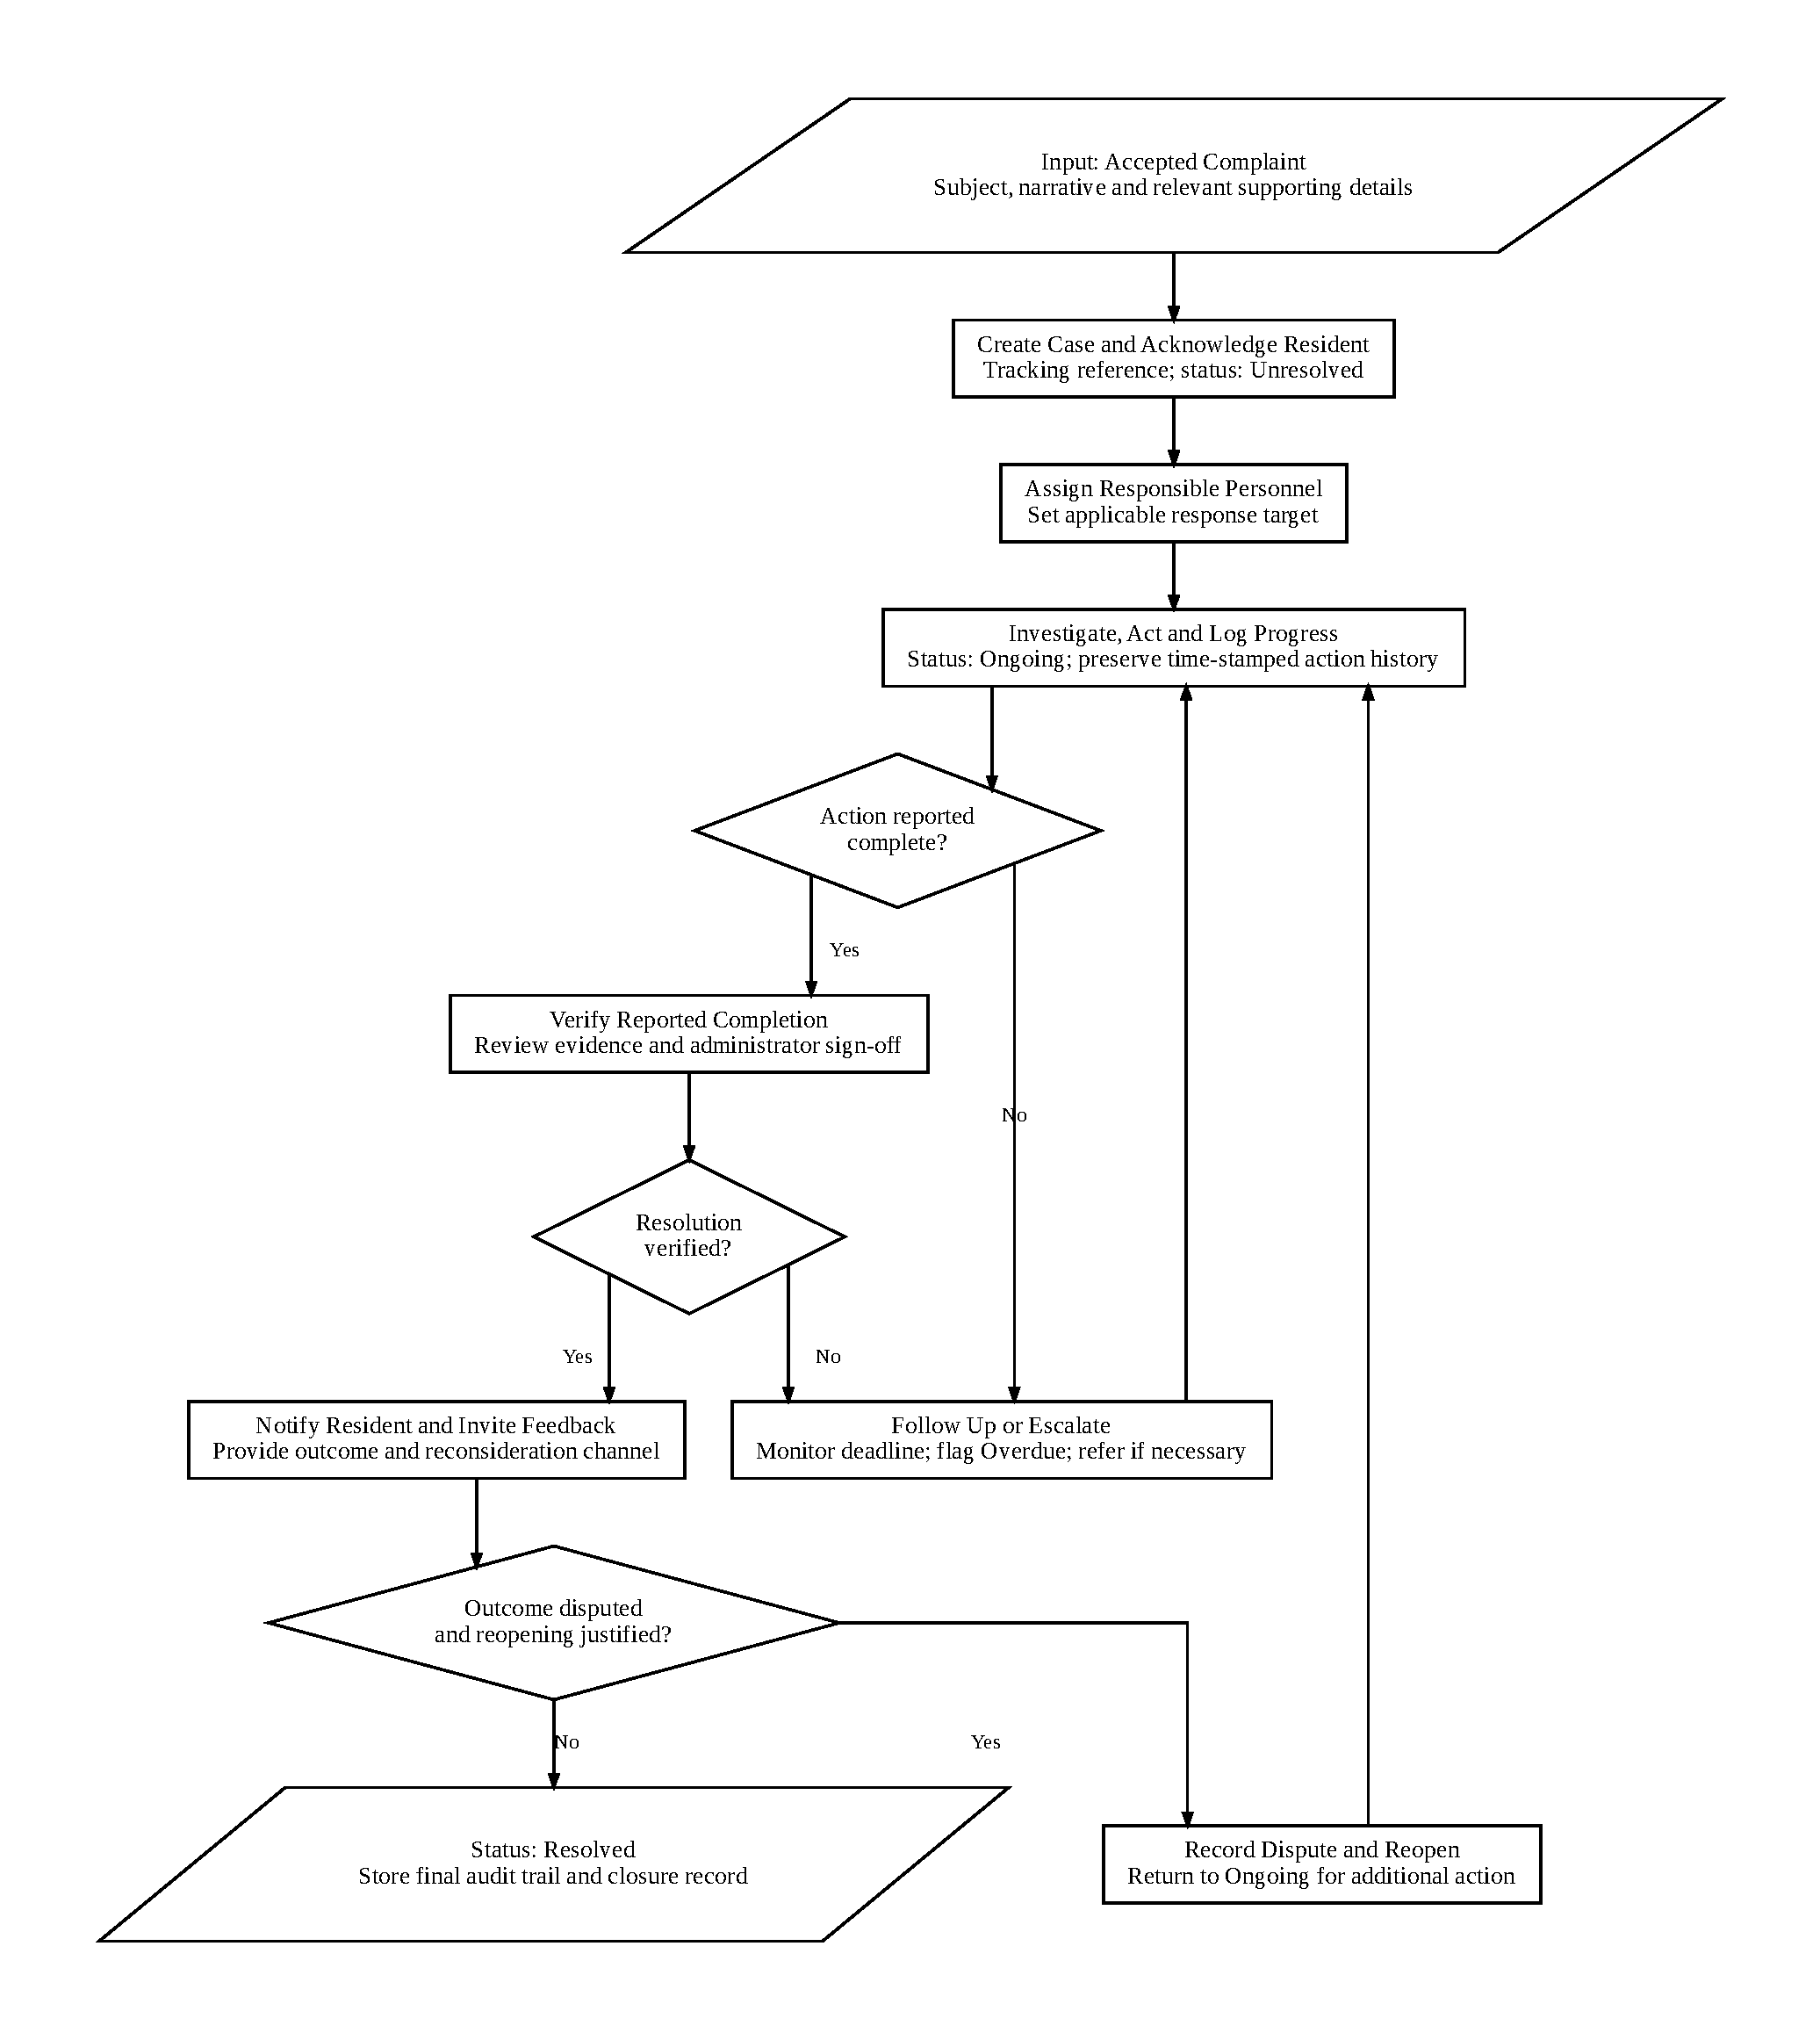
\includegraphics[width=.97\textwidth,height=.87\textheight,keepaspectratio]{figures/case_proposed.pdf}\caption{Proposed accountable complaint case management: accepted-case tracking, action logging, policy-based follow-up, completion verification, resident feedback and justified reopening.}\label{fig:op-case}\end{figure}

\subsection{End-to-End Integrated Complaint Workflow}
The integrated workflow in Figure~\ref{fig:op-integrated} links the previously described modules into one end-to-end account of proposed system behavior. A complaint narrative passes through conservative NLP preprocessing, saved word/character TF--IDF transformers and a calibrated SVM. Predicted Valid narratives proceed to accepted-case management; only predicted Suspicious or Spam narratives enter routine HITL for text-label verification and a separate administrative decision. Reviewed but non-accepted submissions retain a documented clarification or rejection outcome. \emph{Accepted} is an administrative state, not a replacement for the narrative label, while \emph{Resolved} is a later case-management state, not proof that an originally Suspicious sentence was Valid.

The diagram intentionally separates live case handling from the offline learning loop. Case records store assignment, action history, response deadlines and resolution outcomes, whereas versioned human-verified narrative labels are quality-checked before they can enter the training-feedback pool. Training a new TF--IDF--SVM candidate requires a justified and authorized retraining decision; the deployed classifier changes only after successful validation and release approval. In particular, neither an Accept click nor case resolution automatically updates model weights or training labels. These are proposed control boundaries, not additional observed results from the recorded synthetic-data baseline \cite{ra10173,rottger2022,sklearnpitfalls,nist}.
\begin{figure}[H]\centering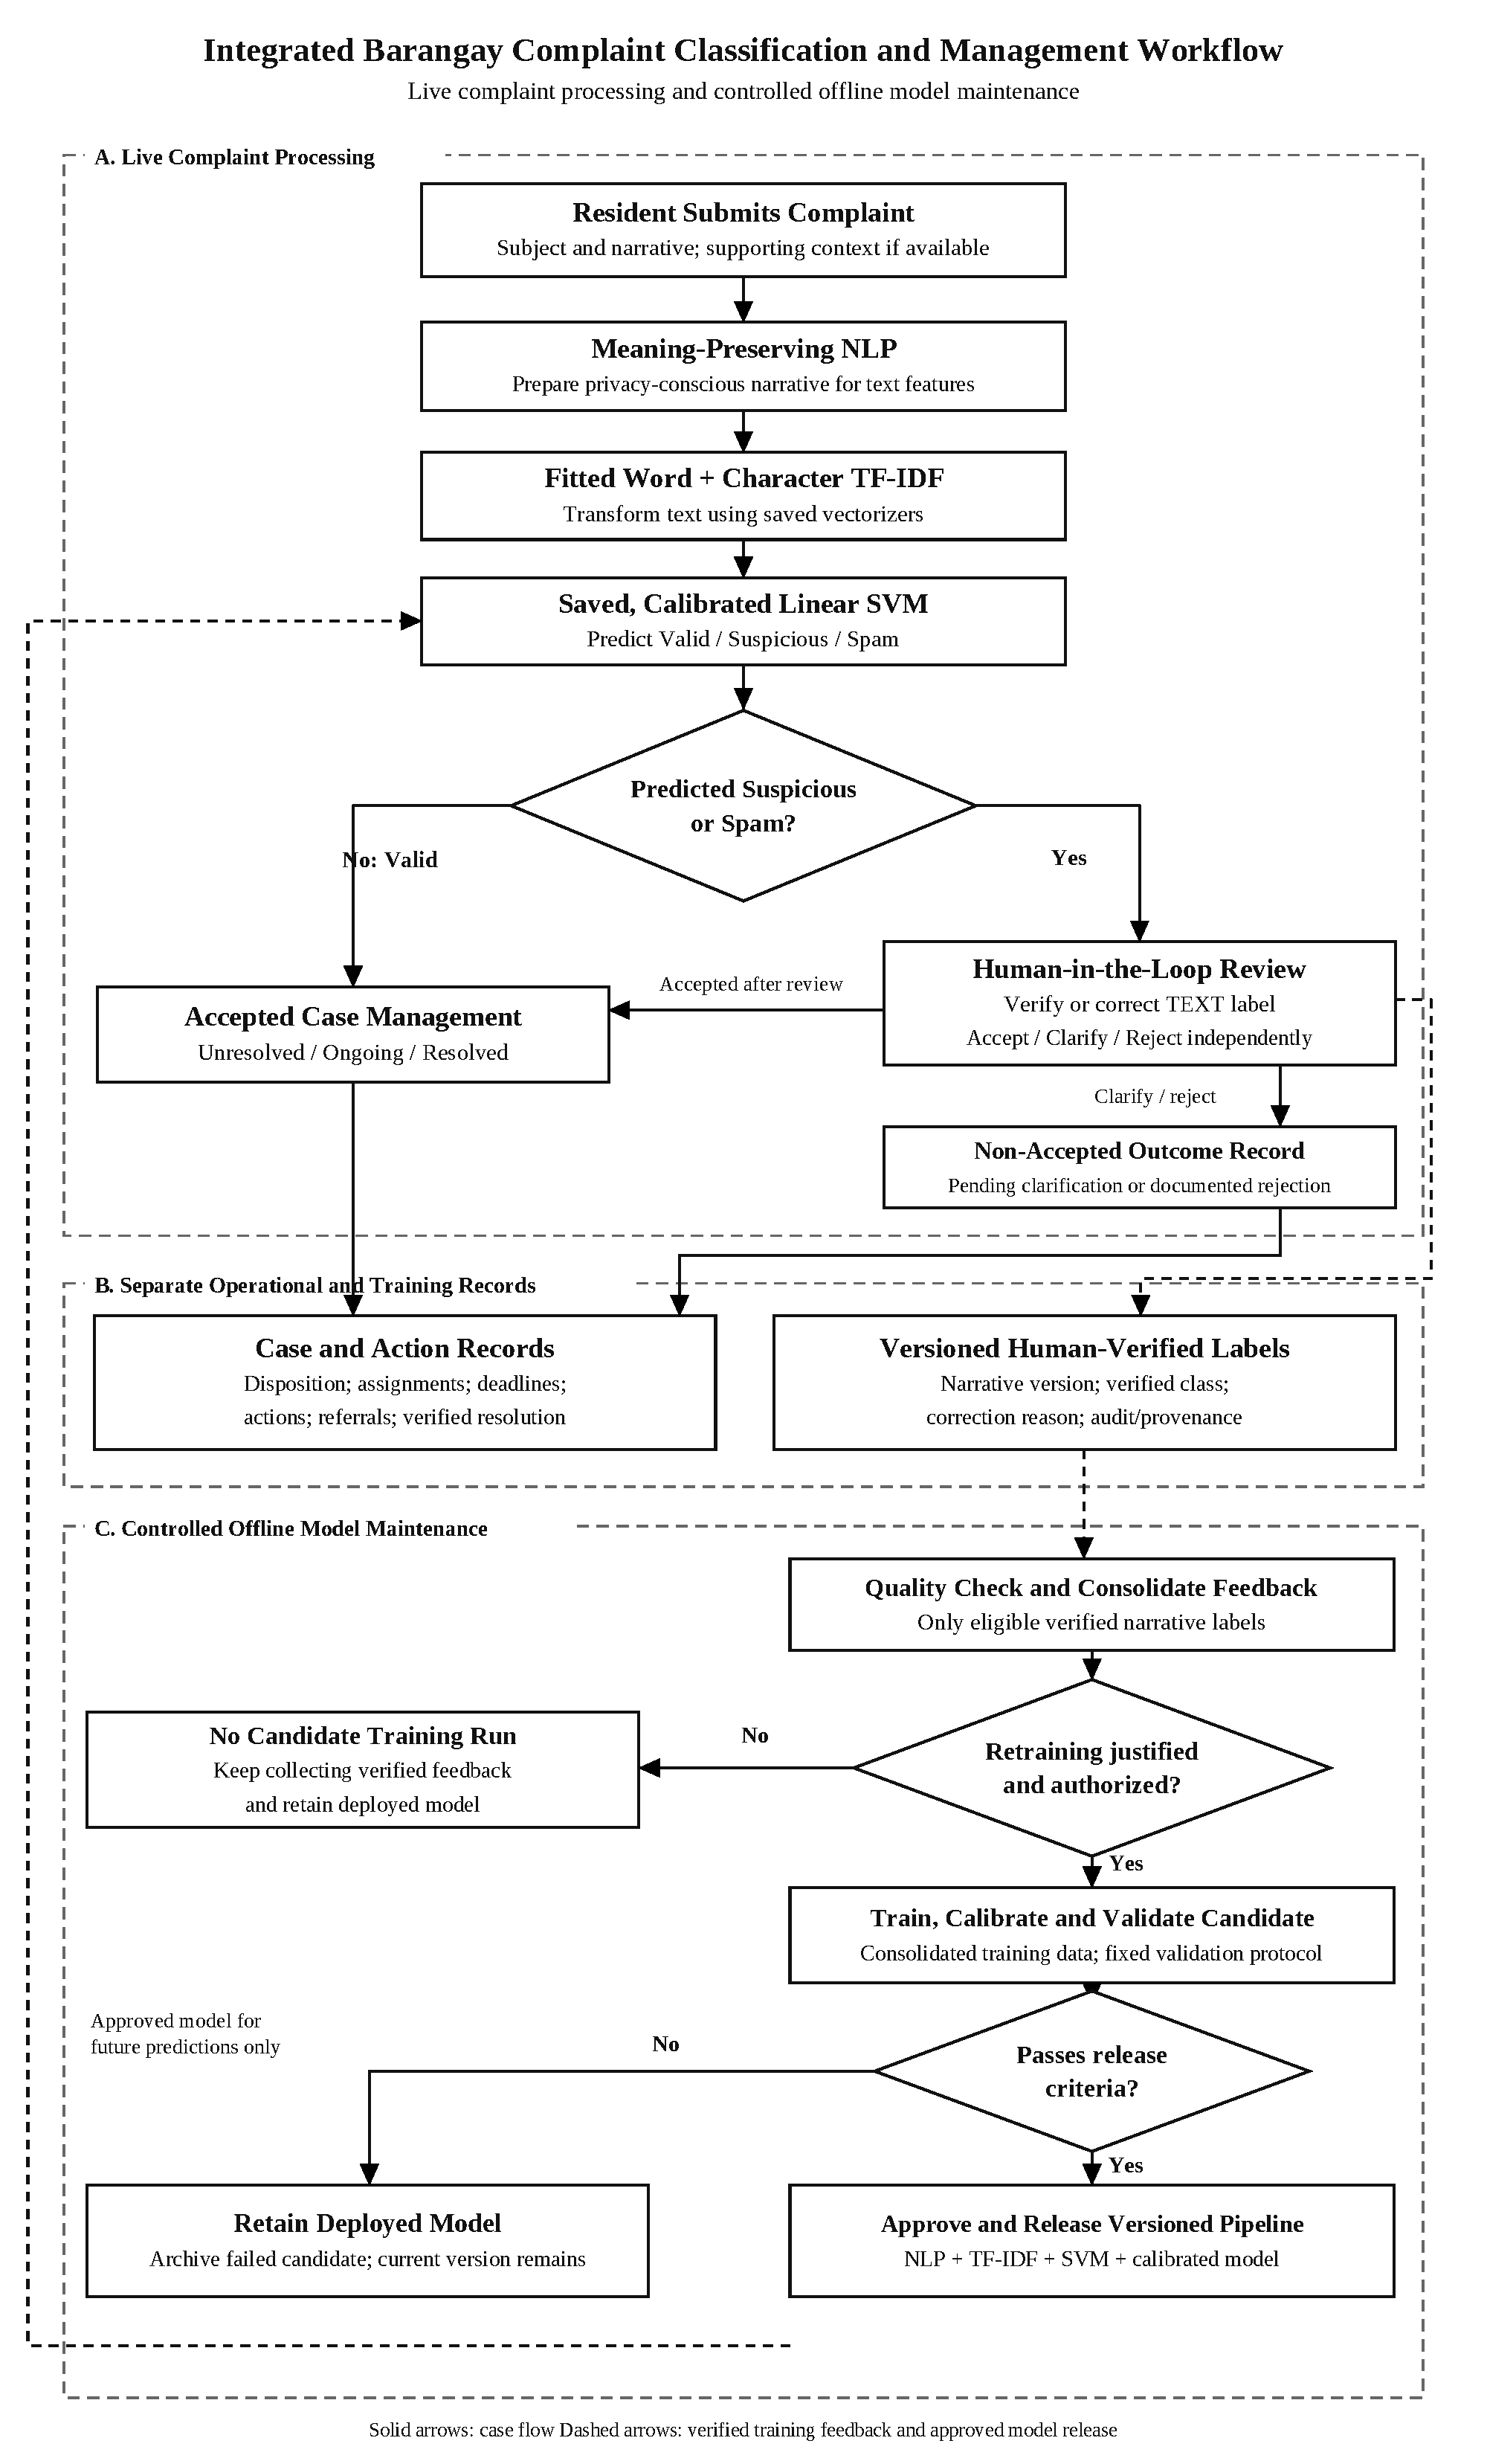
\includegraphics[width=.99\textwidth,height=.87\textheight,keepaspectratio]{figures/end_to_end_workflow.pdf}\caption{Proposed end-to-end integrated workflow connecting resident submission, NLP, TF--IDF, SVM, class-specific human review, accepted-case processing and approved offline retraining. Dashed arrows distinguish training-feedback and approved model updates from live complaint handling.}\label{fig:op-integrated}\end{figure}

\subsection{Software Component Integration and Data Boundaries}
After the end-to-end workflow, Figure~\ref{fig:op-system-integration} presents the complementary \emph{software component integration} and its access boundaries. The proposed resident portal and authorized administrator dashboard exchange data through a FastAPI application layer rather than calling the classifier or writing database records directly. The backend manages access checks, request validation, classification requests, tracking references, administrative actions and auditable case updates. Next.js/TypeScript, FastAPI/Python and PostgreSQL are the suggested application stack; the uploaded reproducibility evidence does not demonstrate deployment of these services.

The text-only inference service consumes the complaint narrative, applies the saved compatible preprocessing and TF--IDF transformations, and returns a saved calibrated SVM's proposed class probabilities. Predicted Valid follows the accepted-case service; predicted Suspicious or Spam enters administrator review. Reviewers may correct the \emph{text label} independently of Accept/Clarify/Reject decisions. Accepted cases and non-accepted submission outcomes share secured persistence but maintain different administrative states, while eligible verified narrative labels are stored as a \emph{distinct feedback dataset}. Later, an authorized offline candidate training run consolidates eligible training records, retrains the feature extractors and classifier, checks calibration and held-out validation, and releases a single versioned model bundle only after approval. The approved release path denotes an approved future inference version, never incremental training during complaint submission. The proposed design excludes photographic inputs and location maps from model inference and does not claim that a completed case is necessarily a Valid textual training example \cite{sklearnpitfalls,sklearncalib,ra10173,nist}.
\begin{figure}[H]\centering
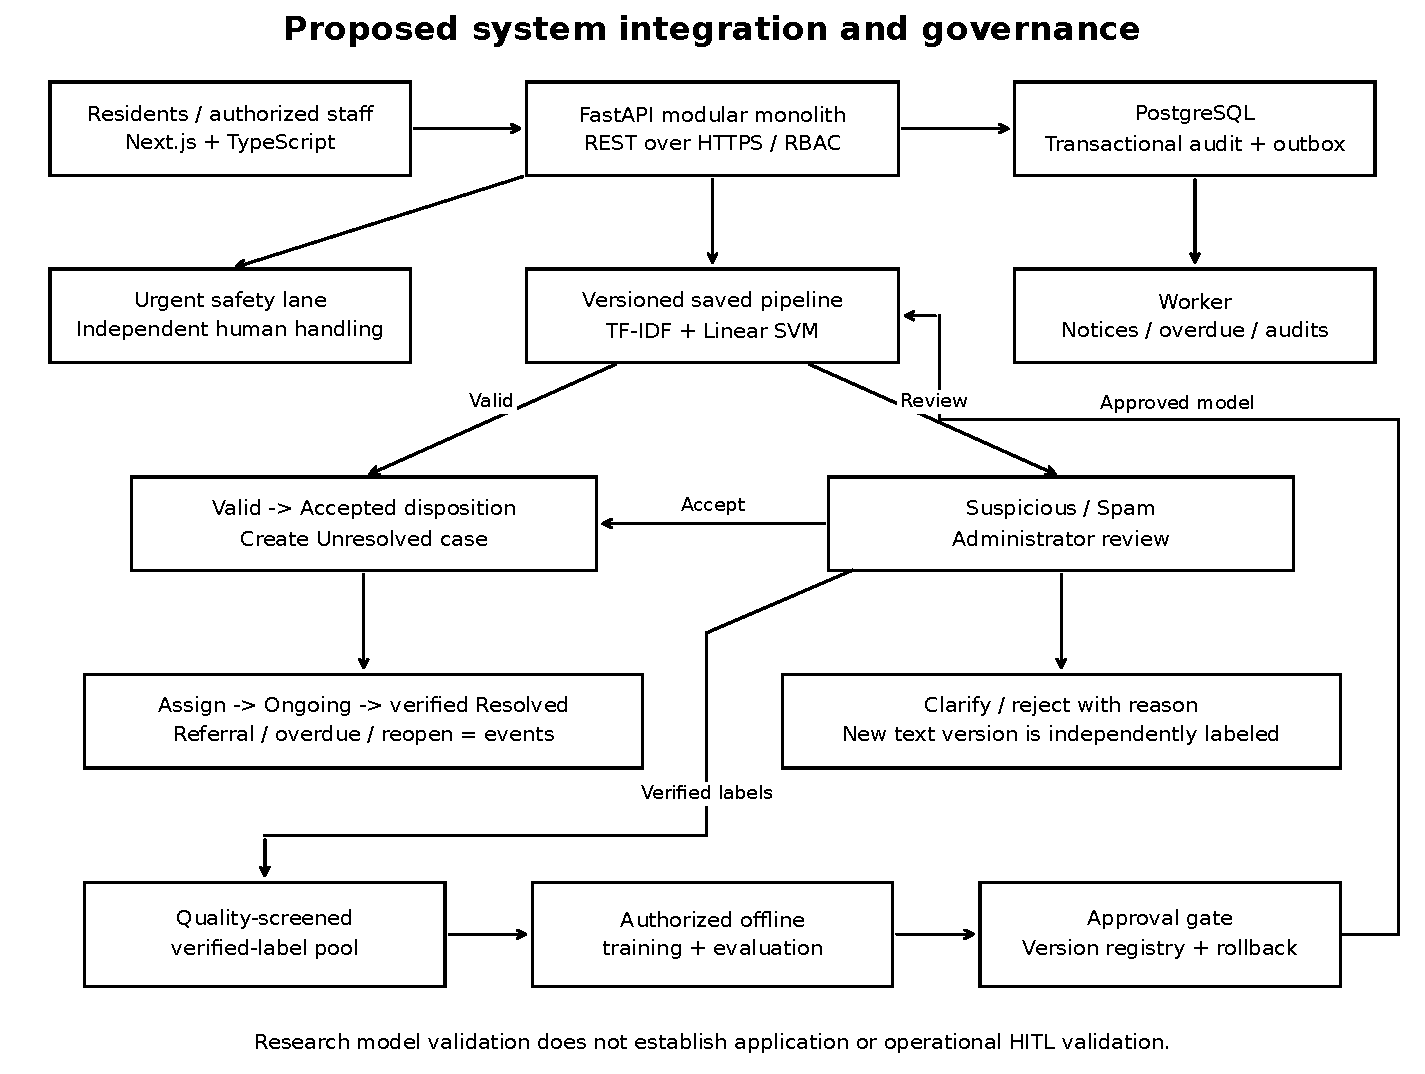
\includegraphics[width=.99\textwidth,height=.84\textheight,keepaspectratio]{figures/verified/system_architecture.pdf}
\caption{Proposed system integration architecture showing the resident and administrator interfaces, application API, text-classification service, HITL review, separate case and feedback records, and controlled offline model-release boundary. The component diagram specifies a target implementation, not a deployed or evaluated full-stack system.}\label{fig:op-system-integration}
\end{figure}

\subsection{Implementation and Evaluation Gates}
\begin{table}[H]\centering\small\caption{Evidence boundary and evaluation required for proposed extensions}\label{tab:op-evidence}\begin{tabularx}{\textwidth}{p{.29\textwidth}Xp{.24\textwidth}}\toprule
Component & What the supplied research currently supports & Required next evidence\\\midrule
24,000-row synthetic dataset & Fixed counts, partitions, metadata and researcher-generated texts; all review flags negative. & Human annotation and authentic external validation.\\
Word TF--IDF + Linear SVM & Recorded group-aware grid/CV and within-generator validation; test generalization remains limited. & Independent test beyond generator patterns.\\
Word + character combination & Reference reproduction and separate combined-feature development experiment. & Independent external comparison beyond the synthetic ceiling.\\
Probability calibration and HITL & Synthetic development calibration; HITL remains a proposed policy. & External probability reliability, reviewer agreement and Valid-sample audits.\\
Human-feedback retraining & Cumulative checkpoints and release-gate plan. & Verified feedback, fixed validation, approved candidate run.\\
Case management/accountability & Flowchart and local legal/interface precedents. & Implemented audit logs, deadlines, referral and resident tests.\\\bottomrule
\end{tabularx}\end{table}

\subsection{Detailed Full-Stack Implementation Plan}
The proposed architecture separates Next.js/TypeScript resident and administrator interfaces, FastAPI inference and workflow endpoints, and PostgreSQL records for versioned narratives, predictions, verified labels, dispositions and accepted cases. Object-scoped authorization, append-only histories, explicit state transitions, and model-release approval are required application controls. Figure~\ref{fig:op-system-integration} supplies the single software-integration overview; Figure~\ref{fig:verified-db} gives the complementary relational model. These are implementation plans, not validation of the existing SQLite/static-HTML prototype. Direct Valid routing records policy-based acceptance but never creates a human-verified label. Urgent human handling is independent of predicted class. The editable diagram sources and detailed schema are maintained in the repository documentation.
The relational design links immutable narrative versions to separate predictions and verified labels; accepted dispositions alone create cases. Append-only action and audit histories preserve the distinction between machine outputs and administrative decisions.

\begin{figure}[H]\centering
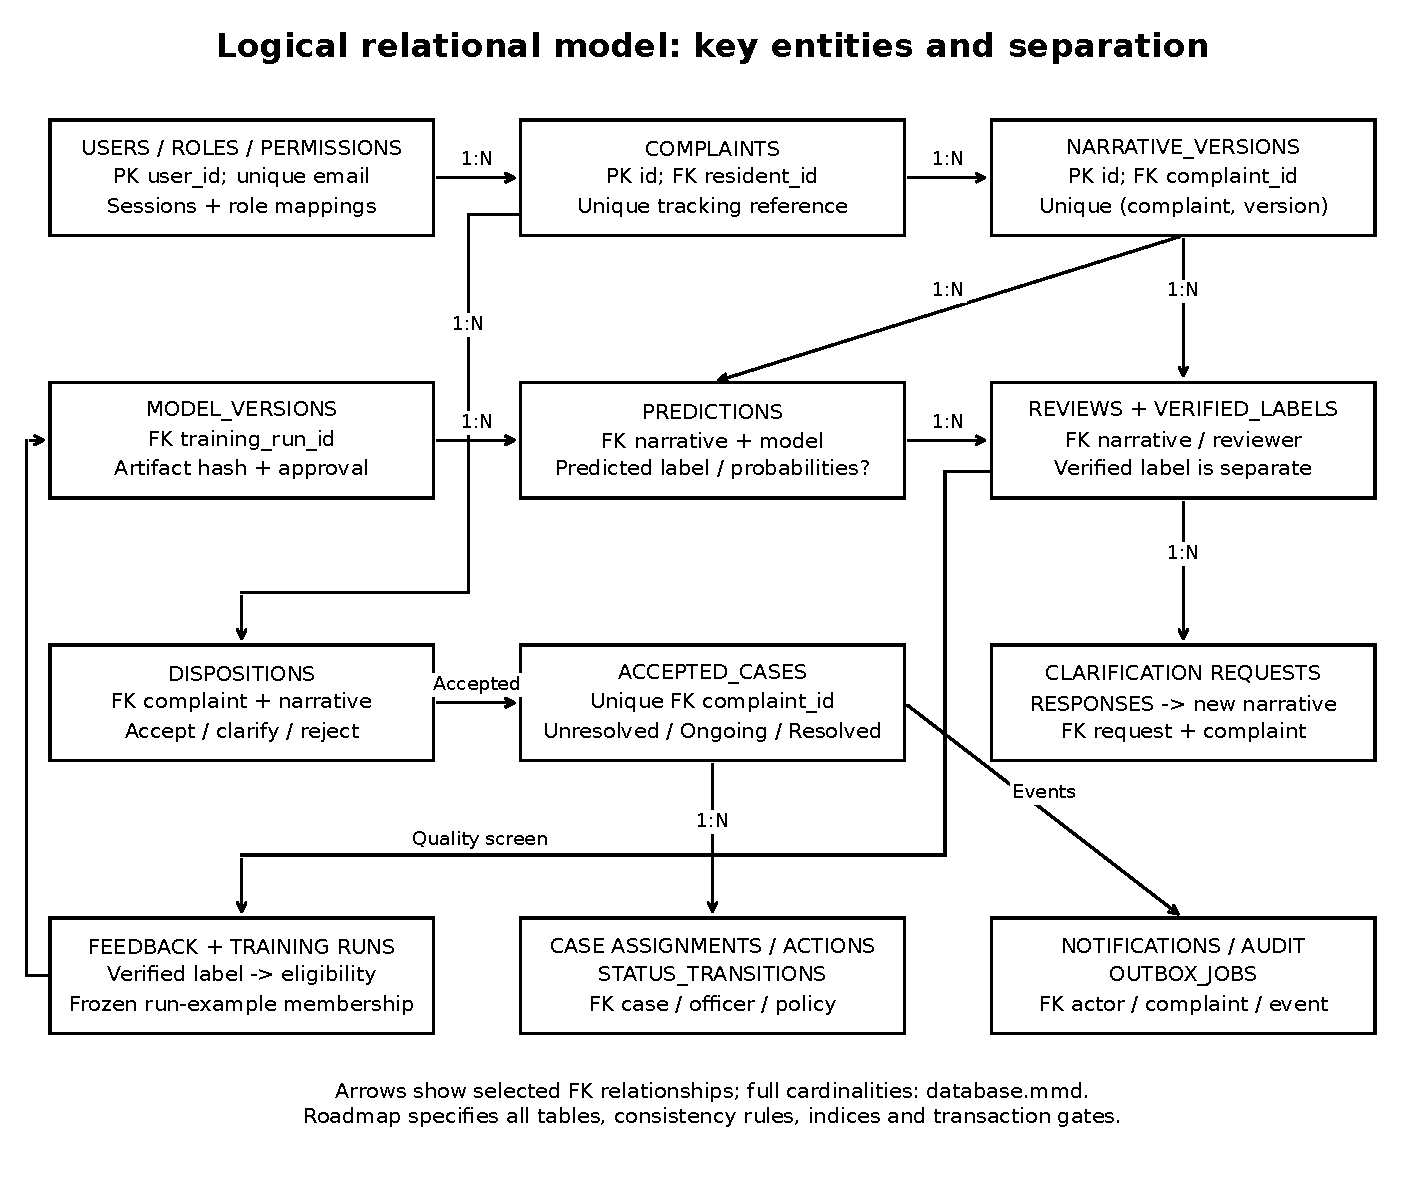
\includegraphics[width=.96\textwidth,height=.70\textheight,keepaspectratio]{figures/verified/database_overview.pdf}
\caption{Proposed logical relational overview; keys, constraints, indices and cardinalities are specified in the repository schema design.}\label{fig:verified-db}
\end{figure}


\section{Research Ethics, Reproducibility and Limitations}
The corpus contains researcher-generated narratives rather than private resident reports. Reproducible inputs include the category register, generator source, random seed, partition CSVs, run records, training scripts and model metrics. Ethical deployment requires privacy-conscious logging and retention, a clear review process, and transparent handling of urgent reports. Because generator-authored patterns remain correlated with class labels, the measured within-generator accuracy can exaggerate transferable performance. No prospective performance gain from Human-in-the-Loop retraining or reduction in office workload is claimed without an implemented and evaluated user study.

\subsection{Separately Evaluated Combined-Feature Candidate}\label{sec:candidate-final}
The candidate is distinct from the original SVM: Unicode NFKC, casefolding and whitespace normalization preserve negations and accented characters; word $(1,2)$ TF--IDF (min\_df 2, max\_df .95) is concatenated with character-within-word $(3,5)$ TF--IDF (min\_df 3, maximum 45,000 features). Both branches use sublinear TF and default L2 normalization, equal weights and LinearSVC $C=.1$. One fixed candidate was evaluated; no new search was performed. A calibrated variant uses sigmoid \texttt{CalibratedClassifierCV} with an ensemble of three precomputed scenario-disjoint training folds, each refitting its complete feature pipeline. Calibration folds do not fit their corresponding base estimators. Existing development validation evaluates the candidates; the historical test was not used for them \cite{sklearncalib,sklearnpitfalls}.

Both variants tied the reference's validation Macro-F1, so no classification improvement is demonstrated. Log loss, multiclass Brier score and ten-bin expected calibration error describe synthetic development probability behavior. These are completed development diagnostics, not independently verified operational calibration. The reference SVM has no calibrated probabilities; routing remains class-based, not an untested probability threshold. Chapter~4 reports candidate findings separately; live calibration approval and external validation remain future work.
